%% FEUP THESIS STYLE for LaTeX2e
%% how to use feupteses (English version)
%%
%% FEUP, JCL & JCF, 31 July 2012
%%
%% PLEASE send improvements to jlopes at fe.up.pt and to jcf at fe.up.pt
%%

%%========================================
%% Commands: pdflatex tese
%%           bibtex tese
%%           makeindex tese (only if creating an index)
%%           pdflatex tese
%% Alternative:
%%          latexmk -pdf tese.tex
%%========================================

%% 2021-07-20: One-sided output by default
\documentclass[11pt,a4paper]{report}
%% For two-sided printing (for dead-tree output) comment previous line
%% and uncomment the next line
%% \documentclass[11pt,a4paper,twoside,openright]{report}

%% For iso-8859-1 (latin1), comment next line and uncomment the second line
\usepackage[utf8]{inputenc}
%\usepackage[latin1]{inputenc}

%% English version

%% MEIC options
%\usepackage[meic]{feupteses}
%\usepackage[meic,juri]{feupteses}
\usepackage[meic,final]{feupteses}
%\usepackage[meic,final,onpaper]{feupteses}

%% MEEC options
%\usepackage[meec]{feupteses}
%\usepackage[meec,juri]{feupteses}
%\usepackage[meec,final]{feupteses}

%% For other degrees
%\usepackage{feupteses} % you must define the degree bellow

%% Additional options for feupteses.sty: 
%% - onpaper: links are not shown (for paper versions)
%% - backrefs: include back references from bibliography to citation place

%% Uncomment to create an index (at the end of the document)
%\makeindex
\usepackage{listings}
\usepackage{amsfonts}
\usepackage{amsmath}
\usepackage{hyperref}
\usepackage{comment}
\usepackage{xurl}
\usepackage{natbib}


%% Path to the figures directory
%% TIP: use folder ``figures'' to keep all your figures
\graphicspath{{figures/}}

%%----------------------------------------
%% TIP: if you want to define more macros, use an external file to keep them
%some macro definitions

% format
\newcommand{\class}[1]{{\normalfont\slshape #1\/}}

% entities
\newcommand{\Feup}{Faculdade de Engenharia da Universidade do Porto}

\newcommand{\svg}{\class{SVG}}
\newcommand{\scada}{\class{SCADA}}
\newcommand{\scadadms}{\class{SCADA/DMS}}

%%----------------------------------------

%%========================================
%% Start of document
%%========================================
\begin{document}

%%----------------------------------------
%% Information about the work
%%----------------------------------------
\title{Meta Feature Classification on a Synthetic Dataset Generator}
\author{João Carlos Fonseca Pina de Lemos}

%% Comment next line if not necessary for degree
\degree{Master in Informatics and Computing Engineering}

%% Uncomment next line for date of submission
%\thesisdate{July 31, 2008}

%% Comment next line copyright text if not used
%\copyrightnotice{Name of the Author, 2008}

\supervisor{Supervisor}{Daniel Augusto Gama de Castro Silva}

%% Uncomment next line if necessary
\supervisor{Second Supervisor}{Leonardo Silva Ferreira}

%% Uncomment committee stuff in the final version if used
\committeetext{Approved by \ldots:}
\committeemember{President}{Rosaldo Rossetti}
\committeemember{Referee}{Pedro Abreu}
\committeemember{Referee}{Daniel Silva}

%% Uncomment signature line in the final on paper version if used
%\signature

%% Specify cover logo (in folder ``figures'')
\logo{uporto-feup.pdf}

%% Uncomment next line for additional text below the author's name (front page)
%\additionalfronttext{Preparação da Dissertação}

%%----------------------------------------
%% Preliminary materials
%%----------------------------------------

% remove unnecessary \include{} commands
\begin{Prolog}
  \chapter*{Abstract}
Machine learning (ML) models can perform a vast amount of tasks. Recognition of images and speech, statistical arbitrage (useful in finance), performing medical diagnostics through the analysis of medical exams, and performing predictive analysis are skills in their repertoire. The ML models must be trained using extensive data to accomplish these tasks.

%Each machine learning model needs to absorb data related to the task it will end up performing, 
Valid data is usually either scarce, expensive, or not readily available. Scrapping tools are commonly used to circumvent the scarceness of data, but their quality is questionable. A small dataset is also insufficient to produce an accurate prediction model. Even in cases where a large amount of data is available, its use may infringe privacy policies (a common problem when entering the medical field). These problems represent an accumulation of problematic data that leads to incorrect results. Synthetic datasets have a proven track record of improving ML effectiveness by providing a better dataset with fewer data imbalances than its "organic" bredren. 

The work developed in this study focus on the study of meta feature extraction methods and meta feature insertion analysis. Using an already existing Ticket-based Synthetic DataSet Generator as a basis, we also developed a meta extractor feature.

Each dataset has its group of meta features - its fingerprint. Our meta feature extractor feature can dissect any kind of CSV tabular dataset, even if those datasets were not synthetically generated by our generator.
%When an existing dataset is available, the generator should analyse it and its meta features extracted, then used as parameters for the generation process. This generation should also be available if no original dataset is provided by making a simple selection of parameters. 
Despite being referenced in many studies, meta features are not uniformly described. Nevertheless, some studies agree on lists of meta features, and those arranged lists are explored. Besides extracting parameters from existing datasets' meta features, it is also essential to analyse the parameter-parameter relationship.
%The quality of the synthetic dataset is also a factor of concern: cases of missing data, imbalances, anomalies and overfitting can easily happen during the generation process, and as such, the number of outliers must be realistic. Outliers should exist in a dataset as they contain useful information.

We also explored the concept of meta feature inclusion in the generation process, where we try to force values of certain meta features into the final synthetic dataset.

%The workflow started with the analysis and definition of a set of meta features, passing to the creation of parameters in the generator corresponding to that same data features. The quality assurance process will be the final step in the practical development of this study.

\vspace*{10mm}\noindent
\textbf{Keywords}: Synthetic Dataset, Meta Features, Machine Learning
 % the abstract
  \chapter*{Agradecimentos \footnote{Unlike the rest of this study, the acknowledgements are written in Portuguese to be read by every person mentioned, some of which are native only speakers.}}

Um trabalho de mestrado é uma longa caminhada, marcada por diversos desafios, incertezas, alegrias e tristezas. Apesar do processo solitário a que qualquer investigador está destinado, o seu percurso é também pautado pelo apoio de várias pessoas, às quais dedico este trabalho. 

Em primeiro lugar, gostaria de exprimir os mais sinceros agradecimentos ao meu orientador, professor doutor Daniel Castro Silva e ao meu co-orientador, Leonardo Silva Ferreira, pela orientação exemplar, rigor científico, disponibilidade e conselhos facultados ao longo dos últimos meses. 

Agradeço aos meus grandes amigos e colegas de curso, Ricardo Figueiredo e Luís Guilherme Neves, por terem sempre puxado por mim e me terem ajudado quando mais precisei – é também graças a vocês que este trabalho é possível. 

Obrigado aos meus amigos Sérgio Pinto, Rahul Pires, João Brandão, João Pedro Morais, Mafalda Neves, Inês Faria e Sara Aguiar por todos os momentos passados e amizade transmitida.  

Um obrigado à Tuna de Engenharia da Universidade do Porto (TEUP) - lugar onde encontrei a minha casa longe de casa, e por ter sido a escola que fez de mim grande parte da pessoa que sou hoje. 

Agradeço à minha terapeuta Dra. Sara Malheiro, pela atenção, disponibilidade, prontidão e amizade que me permitiram trilhar o caminho certo para aqui chegar. 

Ao professor doutor António Augusto Sousa, pelas constantes palavras de encorajamento e por uma conversa especial que fez com que fosse capaz de olhar para este percurso com outros olhos. 

Por fim, e como não podia deixar de ser, dirijo os meus maiores agradecimentos à minha família, que revelou ser o maior porto de abrigo e refúgio nos momentos mais difíceis.  

Aos meus pais, que sempre foram um exemplo de dedicação, trabalho e esforço. 

Ao meu irmão Pedro, meu melhor amigo, com quem partilho memórias e momentos muito felizes.  

Às minhas tias Helena e Elsa, que ao longo da vida (em especial dos anos no Porto) foram sempre a principal rede de apoio e ajuda para tudo, e a quem serei eternamente grato.  

Às minhas tias São, Zeza, e à minha prima Xana pelo carinho e amizade desde sempre.  

À Mariana, um especial e muito grande agradecimento por, mesmo nos momentos mais difíceis, nunca me ter deixado desistir e ter acreditado que tudo isto seria possível. Obrigado pelo carinho, dedicação e amor ao longo dos últimos nove anos.  
\vspace{10mm}
\flushleft{João Carlos Lemos}
  % the acknowledgments
  \cleardoublepage
\thispagestyle{plain}

\vspace*{8cm}

\begin{flushright}
  \textsl{“The story so far:\\
In the beginning the Universe was created.\\
This has made a lot of people very angry and been widely regarded as a bad move.”}\\
\vspace*{1.5cm}
    Douglas Adams, The Restaurant at the End of the Universe
\end{flushright}
    % initial quotation if desired
  \cleardoublepage
  \pdfbookmark[0]{Table of Contents}{contents}
  \tableofcontents
  \cleardoublepage
  \pdfbookmark[0]{List of Figures}{figures}
  \listoffigures
  \cleardoublepage
  \pdfbookmark[0]{List of Tables}{tables}
  \listoftables
  \chapter*{Abbreviations}
\chaptermark{ABBREVIATIONS}
%\chapter*{Acrónimos}
%\chaptermark{ACRONIMOS}


\begin{flushleft}
\begin{tabular}{l p{0.8\linewidth}}
DT & Decision Tree\\
GUI & Graphical User Interface\\
ML  & Machine Learning\\
MLM & Machine Learning Model\\
PCA & Principal Component Analysis\\
PET & Privacy-enhancing technologies\\
SD & Synthetic Dataset\\
\end{tabular}
\end{flushleft}  % the list of abbreviations used
\end{Prolog}

%%----------------------------------------
%% Body
%%----------------------------------------
\StartBody

%% TIP: use a separate file for each chapter
\chapter{Introduction}
\label{chap:intro}

\section*{}
Dataset is the name given to a collection of related, discrete items of associated data. The Oxford Dictionary defines the term as "a collection of related sets of information that is composed of separate elements but can be manipulated as a unit by a computer.." This data may be accessed apiece, in combination or handled as a complete entity \citep{akhter2019cyber}. The information is typically obtained from historical observations. However, good data is time-consuming, complicated or expensive to acquire \citep{Kar_2019_ICCV}. Synthetic datasets created by a dataset generator are used to combat that problem, making data with similar or better results than organic datasets \citep{anantrasirichai2019deep, Arvanitis2021.02.11.21250741}. SNOOKER is one such generator.

SNOOKER: A DataSet GeNeratOr fOr HelpdesK SERvices is a software program developed initially by Leonardo Ferreira (Second Supervisor) for his doctorate dissertation. As the name implies, this software is responsible for generating datasets for helpdesks. The generator can forge realistic ticket-based datasets that can be used to train intelligent systems. However, several improvements can be made to the current program. Its output should be analysed to extract the dataset's characteristics. To decide on further steps, we will explore the concept of dataset generation further. In the next section, a historical overview and the motivation for the development of this thesis will be explored.

\section{Context and Motivation}
Machine learning (ML) is a data analysis technique that automates analytical model building. It is a branch of artificial intelligence based on the presumption that systems can learn from data, identify patterns and make decisions with the minimal human intervention \citep{wong2021use}. It is, in part, based on a model of brain cell interaction. The term was coined by Donald Olding Hebb in 1949.

\begin{quote}
  ``When one cell repeatedly assists in firing another, the axon of the first cell develops synaptic knobs (or enlarges them if they already exist) in contact with the soma of the second cell.''~ - \cite{hebb1949organisation} 
\end{quote}
%This model describes the interaction between the artificial neurons of the brain model and their changes. These artificial neurons are currently and commonly expressed as \textit{nodes}. \textit{Weight} represents the strength of the relationship between two nodes. Those are the terms that we are going to use subsequently. The weight between two nodes increases if those nodes are activated simultaneously while decreasing when started at different instances.

Evolution resulted in machines capable of processing data using a structural model of the Real World as the basis. These machines used mathematical models and algorithms and ended up not learning but, in fact, merely following instructions \citep{cohen2021evolution}. The next step was to create instructions that allow the computer to learn from experience using the previous model. The machine must be able to extract its own rules from large amounts of data and use those rules for classification and prediction.

Dataset is a term used to describe a collection of data. Data is usually represented in tabular form, making datasets collections of one or more tables. Table columns symbolise a certain variable, and rows relate to the conveyed values of the dataset in question \citep{priyanka2016analysis}. The dataset lists values for each variable for each data set member. Datasets can also consist of a collection of documents or files \citep{snijders2012big}. The dataset description is consensual among the scientific community that uses data as a basis for research activities \citep{renear2010definitions}. As data differs, datasets also differ, having different characteristics. Several studies were made to examine these characteristics and recognise patterns \citep{reif2014automatic}. This topic is further detailed in Chapter \ref{chap:mf}.

Scrapping and collection tools are commonly used to circumvent the scarceness of data. Still, their quality is questionable and highly dependent on the data compilation techniques and annotation procedures \citep{9074205}. 
Challenges still arise when more large-scale datasets are collected. Small datasets are not as effective in producing accurate prediction models, needing further treatment until their use is valid \citep{lateh2017handling}. Problems do exist even in cases where a large amount of data is available. Its use may infringe privacy policies (a common problem when entering the medical field as \cite{s19051181} described in their studies).
These problems represent an accumulation of problematic data that leads to incorrect results \citep{10.1145/3158346}. 
Early works on Synthetic datasets (SDs) were used to fill in missing values in surveys \citep{rubin1986basic}. Nowadays, SDs have a proven track record of improving ML effectiveness by providing a better dataset with fewer data imbalances than its "organic" bredren \citep{anantrasirichai2019deep, Arvanitis2021.02.11.21250741}.

Currently, SDs are used in various fields, ranging from the previously mentioned medical to many others. \cite{anantrasirichai2019deep} used SDs to train a Machine Learning Model (MLM) to pinpoint surface deformation with a strong statistical link to a volcanic eruption. \cite{yu2011geo} looked at increasing social media connection by training an MLM with SDs to group personally and geographically close users, increasing the potential for real-world relationships to flourish. \cite{sethi2017sms} and \cite{hamsapriya2011spam} used them to detect Spam messaging in SMS and email, respectively. \cite{kumar2018comparative} looked at predicting stock market trends using SD-trained MLM. As we can see, the applications of SDs are numerous, making SDs an excellent alternative to real data. 

Meta-learning supports the recommendation of machine learning algorithms and their configurations. These recommendations are based on meta-data, consisting of performance evaluations of algorithms and characterizations of prior datasets. These characterizations, also called meta features, are important metrics to study and will be the focal point of this study.

SDs that use real data, replicating its features in the generation process, have better results. The dynamics and intricacy of real-world systems are practically impossible to be modelled in generators. \cite{6890935} called the process of generating such datasets "Semi-synthetic Data Generation".

While the study of dataset generation is growing (Fig. \ref{fig:sdpapers}), there are still many ways to study, explore and improve the process of SD generation, be it theoretical (through the definition of a set of core meta feature lists) or practical (by looking at generation and evaluation processes). Through the development of this study, we strive to add something to the field.

\begin{figure}[t]
  \begin{center}
    \leavevmode
    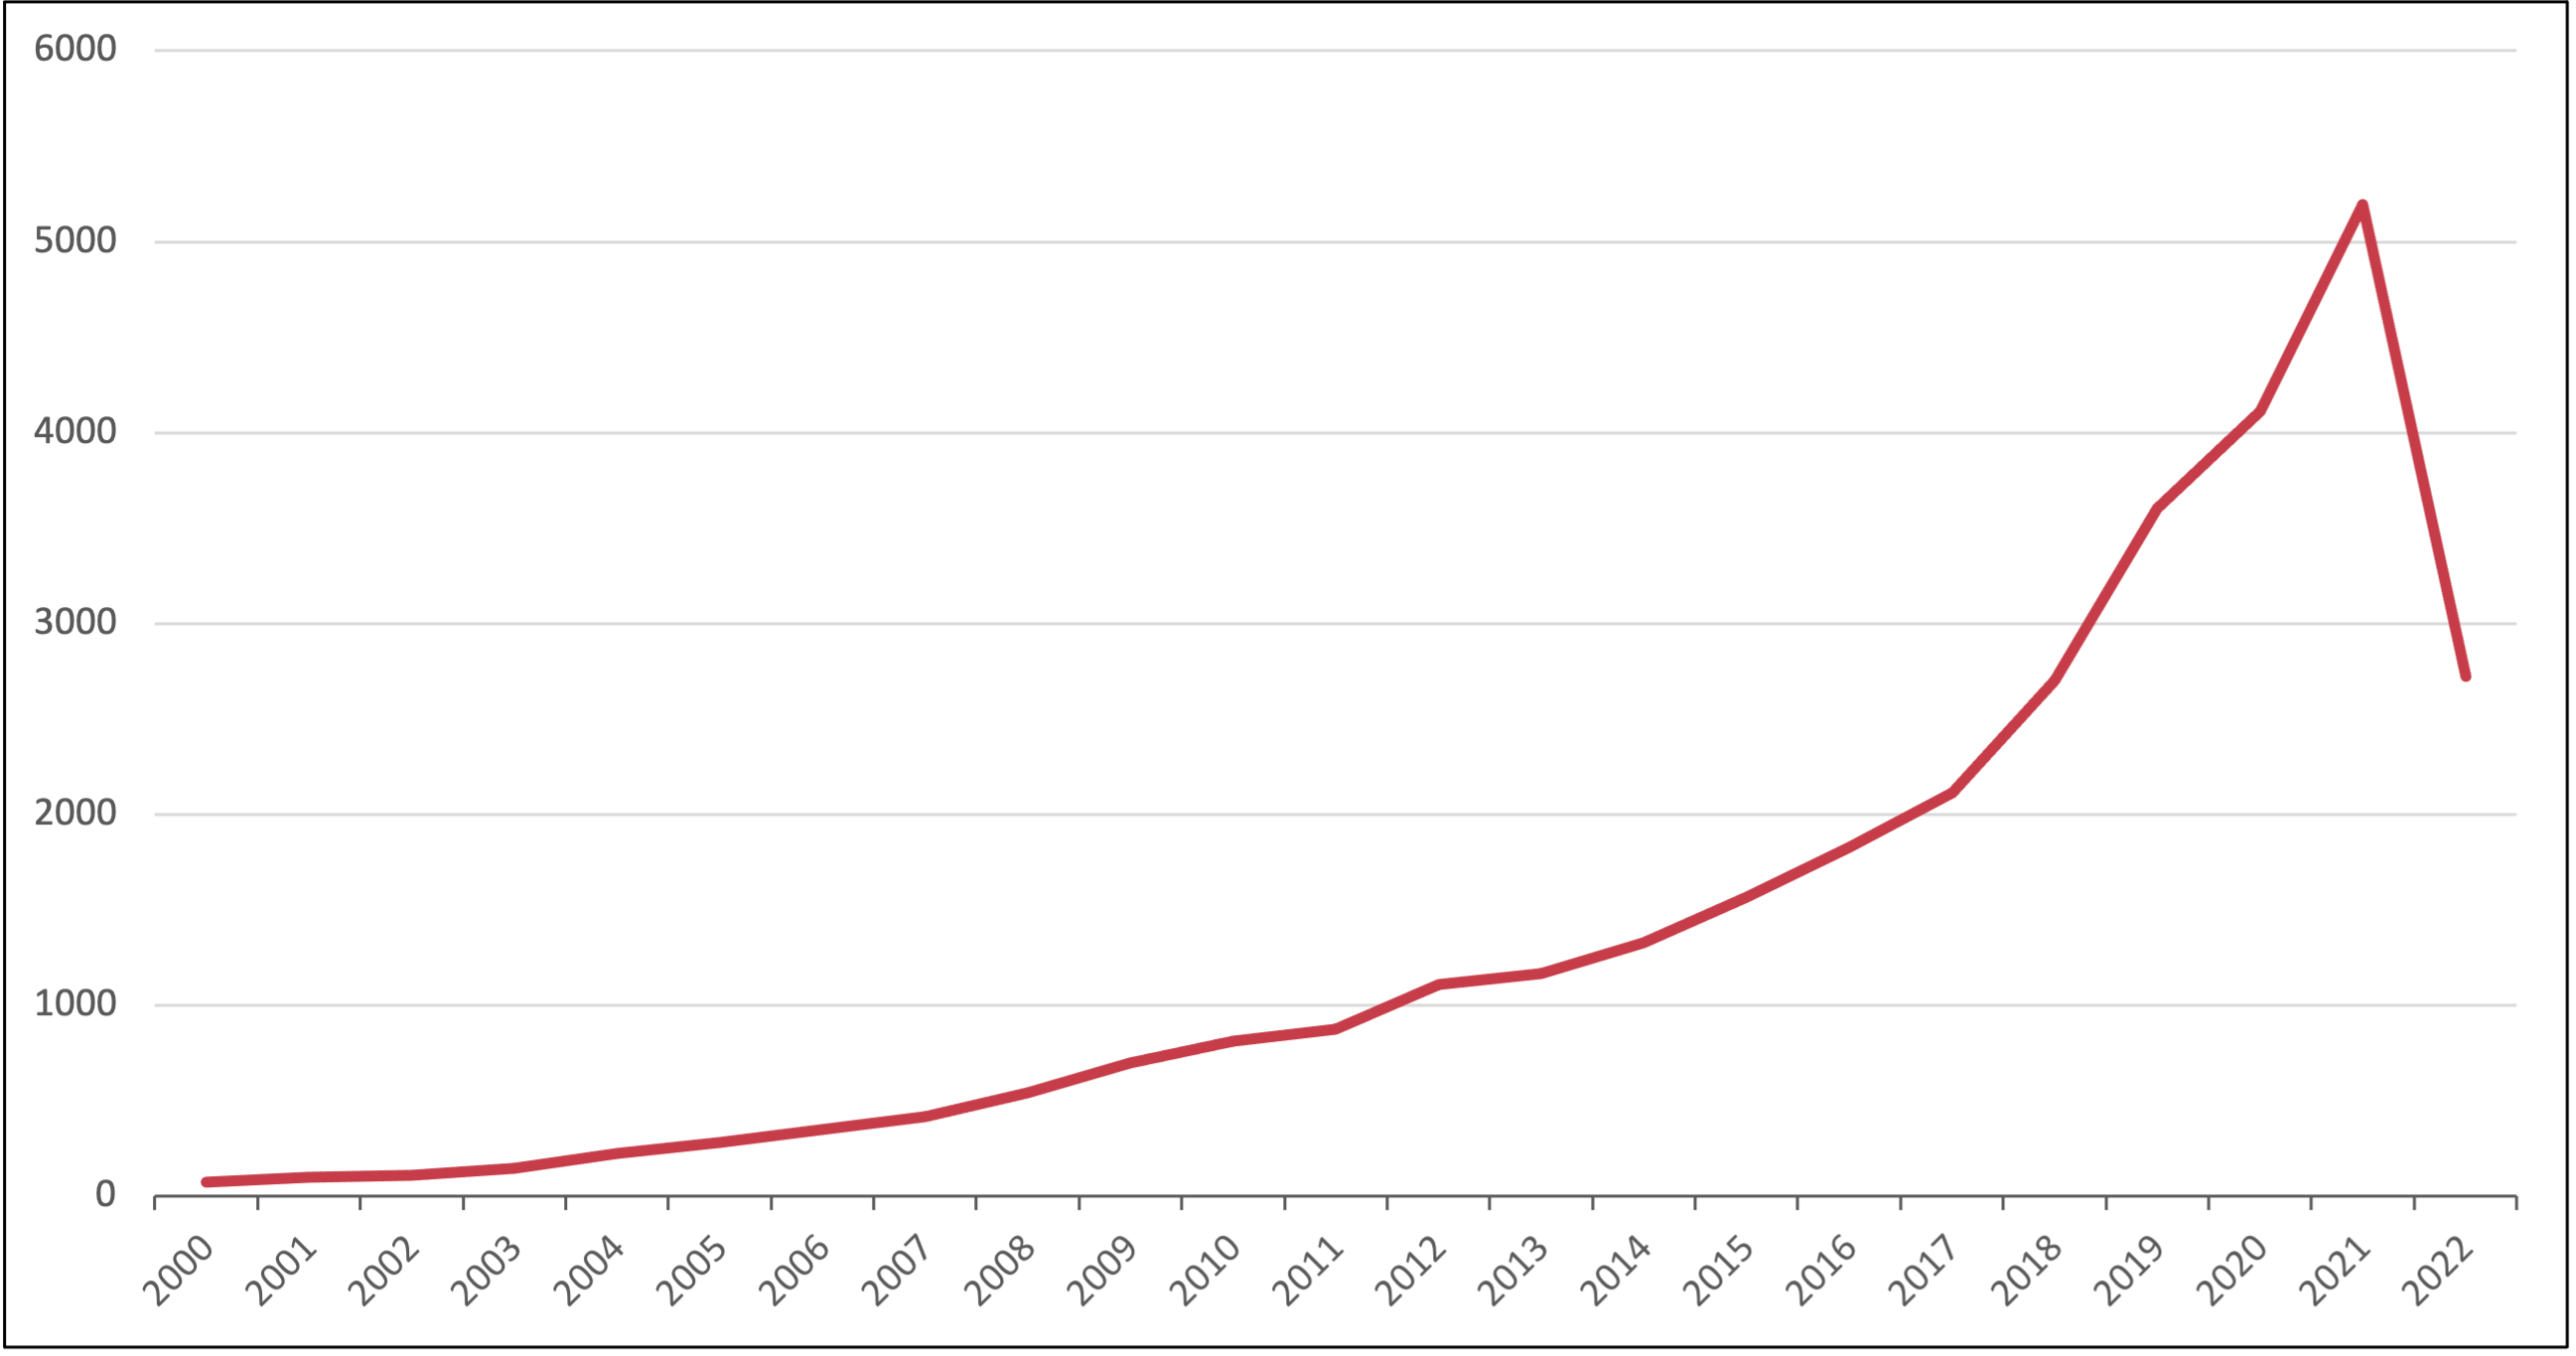
\includegraphics[width=0.8\textwidth]{scopus_sd.png}
    \caption[Number of Synthetic Dataset related papers published on Scopus from 1990 to June 2022]{The number of SD papers published on Scopus from 1990 to June 2022. Data was collected by searching papers using "Syntetic Datasets" as keywords and applying a yearly filter.}
    \label{fig:sdpapers}
  \end{center}
\end{figure}

%\begin{figure}
%    \centering
%    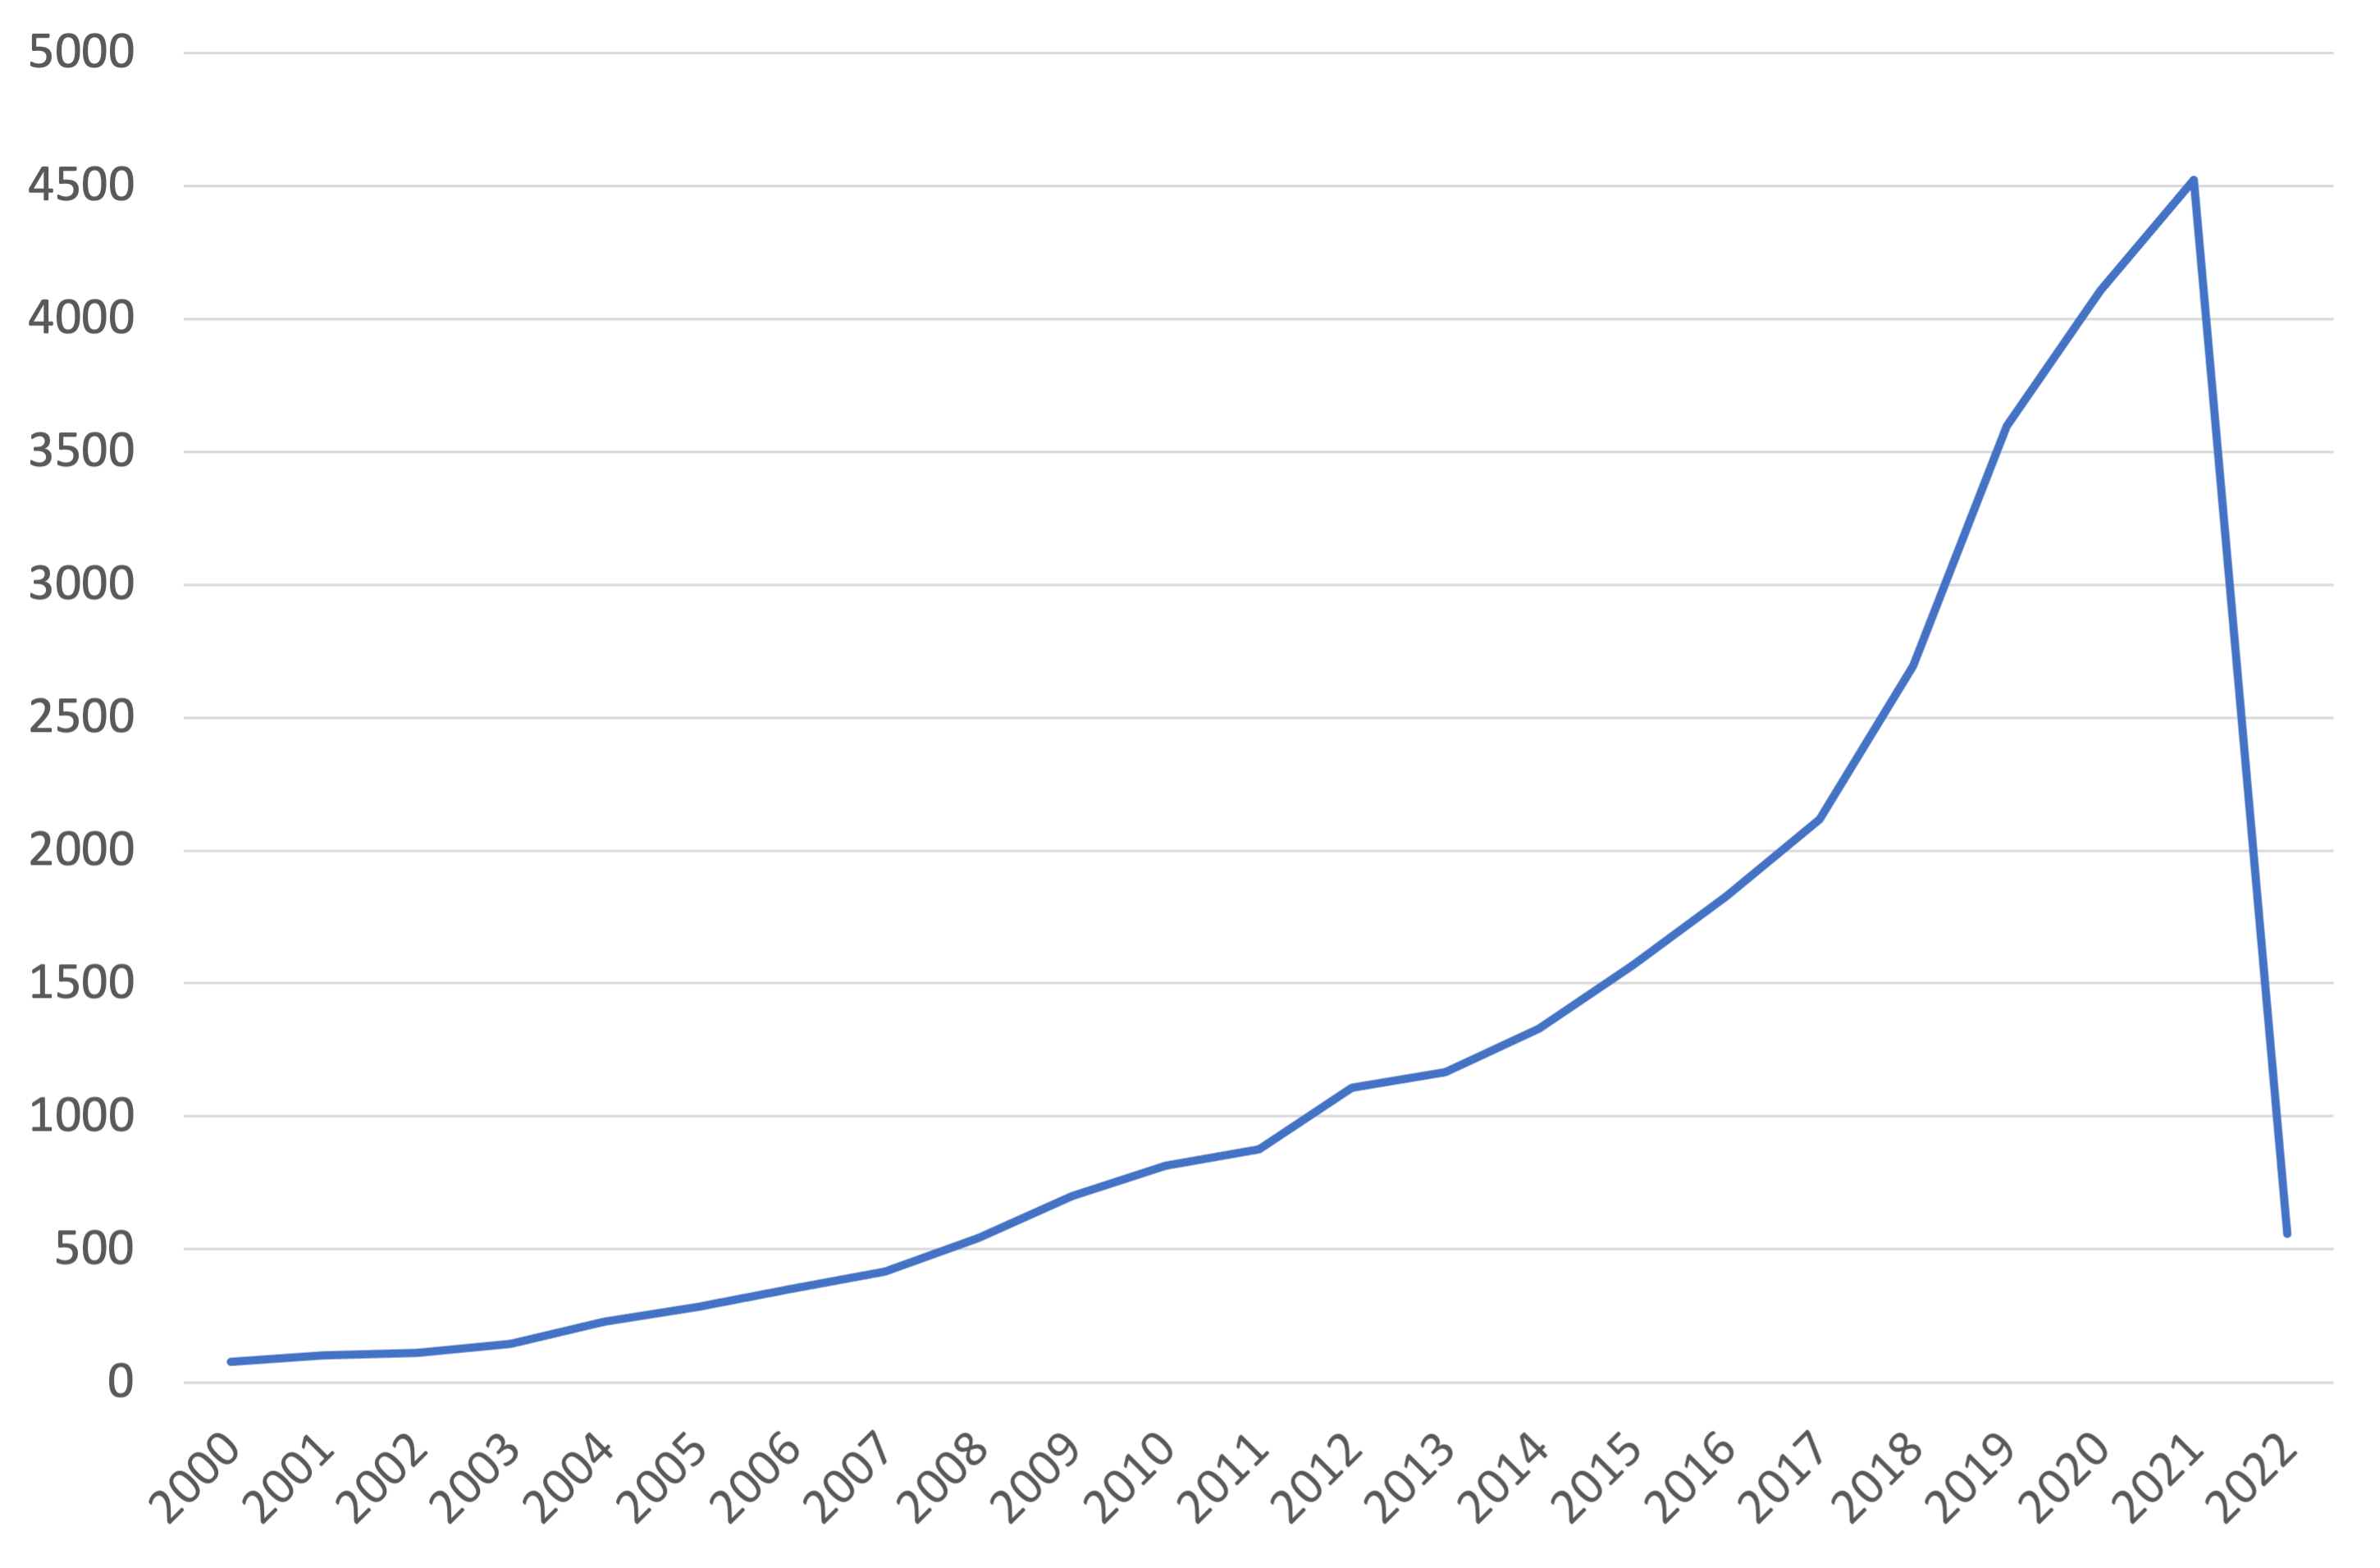
\includegraphics[width=0.8\textwidth]{synteticdatasetstudies.png}
%    \caption{Number of SD papers published on Scopus from 2000 to February 2022. Data was collected by searching papers using "Syntetic Dataset" as keywords and applying a yearly filter}
%    \label{fig:my_label}
%\end{figure}

\section{Objectives}
The work developed in this study is related to enhancing an already existing Ticket-based SD Generator for Helpdesk purposes. We will examine the output dataset and study it, extracting its meta features. We will also explore the possibility of integration of meta features inside the generation process. The aim of this study is both theoretical and practical and will try to answer a series of questions:

\begin{enumerate}
  \item What selection of meta features should be calculated from the data in the synthetic dataset?\\
  This task started theoretically; a list of meta features was made, and selected meta features were included in a meta feature extraction module.
  \item What generation methods can we use?\\
  Collection of generation algorithms followed by analysis and application of the most suitable process to the generator.
  \item Can we include specific values of meta features inside the generation process?\\
  Evaluation of methods to cause certain values of specific meta features inside the generation process. We also study the utility of datasets that go through such methods.
  \item What features can be applied to the generator?\\
  Analysis of the generator and development of new features and improvements.
\end{enumerate}

At the end of this study, we should have a complete set of meta features collected through bibliographic analysis. We will then use this meta feature list as metrics to be extracted from a dataset, letting us fully characterise it through meta-extraction. We should also be able to understand ways to insert some meta feature values into the generation process.

\section{Document Structure}
In this chapter, we looked at the context, motivation, and application of SDs. We also described the objectives of exploring and enhancing the current Ticket-based Synthetic DataSet Generator.

Chapter \ref{chap:mf} will look at the characteristics of datasets and meta features. We will analyze how the inclusion of meta feature selection during the generation process can enhance the creation of a more suitable dataset for the ML process.

In Chapter \ref{chap:generation}, we will explore the process of generating a synthetic dataset. This will be done by investigating some commonly used algorithms and reviewing how other SDs generation projects performed their generation undertakings. We will also look at methods for evaluating the quality of a dataset. These Chapters are part of the state-of-the-art review. 

In Chapter \ref{chap:Problem} the planning for the development of the study will be probed. Close examination of needed tasks will take place. Expected results and validations will also be analyzed. Due to the nature of the study, we will also present a risk analysis in this chapter. The current state of our generator will be studied in Section \ref{chap:Snooker}. We also provide a simplistic outline of SNOOKER and SNOOKER's output.

Chapter \ref{chap:class} will focus on the meta feature classification of synthetic datasets. We will analyse and present the methodology needed to develop this feature.

A critique of the concept of meat feature inclusion during generation is made in Chapter \ref{chap:Integration}.

Finaly in Chapter \ref{chap:Conclusion} we display our final remarks. 
\chapter{Meta Features}
\label{chap:mf}
%The prefix ‘meta’ is of Greek origin and means ‘among’, ‘after’, ‘beside’ or ‘with’.
%Meta-features, describe properties of the data which are predictive for the performance of machine learning algorithms trained on them.
%Feature subset selection (FSS) plays an important role in the fields of data mining and machine learning. A good FSS algorithm can effectively remove irrelevant and redundant features and take into account feature interaction. Although a large number of FSS algorithms have been proposed, there is no single algorithm which performs uniformly well on all feature selection problems. The most commonly used meta-features are established focusing on the following three aspects of a data set: i) general properties, ii) statistic-based properties, and iii) information- theoretic based properties
%The meta-features, also called characterization measures, are able to characterize the complexity of datasets and to provide estimates of algorithm performance.
%The definition of a dataset is a simple one. Datasets are collections of data; as data differs, datasets also differ, having different characteristics. Several studies were made to examine these characteristics and recognise patterns\cite{reif2014automatic}. 
Datasets are data collections; as data differs, datasets also change, having different characteristics. The 'meta' prefix is of Greek origin and means 'among,' 'after,' 'beside' or 'with,' and is often used to identify something that provides information about something else, naming the collection of those characteristics inside the datasets meta features \citep{binder2015analysis}.

Several authors have studied meta features \citep{reif2014automatic}. However, a uniform description of meta features does not exist. Many studies diverge on selecting characteristics to construct their meta feature definition \citep{rivolli2019characterizing}. The reproduction and comparison of said studies are therefore complex and abstract. A meta feature should not be too difficult to calculate \citep{10.1007/11526018_45}.

Meta features are helpful when looking at MLMs as they depict properties of the data, which are predictive of ML algorithms' performance \citep{9640223}. By choosing datasets with a particular assortment of meta features, more valuable data will be analyzed and processed, reducing the use of irrelevant and redundant data.
%One of the main challenges faced when studying meta-features is there forth identified.

Several studies use simple datasets or only focus on purely mathematical distribution-based datasets. While mathematical meta features are valuable \citep{KANDA2016393}, even if datasets with those exact meta features had positive results when applied to the corresponding studies, the same does not apply to a generator. A generator containing only a selection of simple meta features would not be helpful for most cases.

However, analysis of several studies revealed some, even if small, agreeance on some datasets commonly used. It led to the extrapolation of three families: general, statistic-based, and information theoretic-based meta features \citep{reif2012dataset, DBLP:journals/corr/WangSSZXZ14}. General meta features can be directly observable from datasets, statistical use mathematical distributions to describe data distribution, and information-theoretic uses data entropy. Some other studies also included the model-based (usually based on properties of decision trees) and landmarking (use the performance of fast and straightforward learning algorithms to characterize datasets) families \citep{rivolli2019characterizing, 7382962}. In this chapter, we took a look at various sets of commonly used meta features, creating a collected list of features that can be useful in analyzing datasets. %The main objective is to collect and present a list of meta-features to be used later during the development phase of this study. 

\section{General Meta Features}

\begin{table}[h!]
\centering
\caption{General Meta Features}
\setlength{\tabcolsep}{8pt}
	\renewcommand{\arraystretch}{1.2}
    \begin{tabular}{ll}
    \hline
    Acronym & Meaning  \\ \hline
    nrAttr & number of attributes \\
    nrBin & number of binary attributes \\ 
    nrCat & number of categorical attributes \\
    nrNum & number of numeric attributes \\
    numToCat & proportion of numerical to categorical attributes\\
    catToNum & proportion of categorical to numerical attributes \\
    nrInst & number of instances\\
    nrClass & number of classes\\
    attrToInst & proportion of number of attributes to number of instances\\
    instToAttr & proportion of number of instances to number of attributes\\
    classToAttr & number of classes per attribute\\
    instToClass & number or instances per class\\
    freqClass & frequency of instances in each class\\
    nrAttrMissing & number of missing attributes\\
    nrInstMissing & number of missing instances\\
    nrMissing & total missing number \\
    \hline
    \end{tabular}
\label{tab:general-mf}
\end{table}

General meta features are directly observable from the dataset, representing basic information and being the most explicit set regarding computation cost. To a certain extent, they are devised to estimate the complexity of the problem related to that dataset \citep{bilalli2017predictive}.

The measures suggested in Table \ref{tab:general-mf} represent concepts connected to the number of predictive attributes, instances, target classes, and missing values. These measures are relevant to illustrating a dataset's main aspects, delivering knowledge that can support the selection of a dataset for a particular learning task. Most of these measurements are self-explanatory.

It should be explained that the \textit{nrAttrMissing} and \textit{nrInstMissing}, although looking similar, represent different aspects of the same problem. \textit{nrAttrMissing} represents the number of empty columns in a dataset, counting the currently missing attributes. \textit{nrInstMissing} on the other hand, represents the number of entries (rows) that are empty.

While most meta features are synonymous with a straightforward examination, others can provide additional connotation: \textit{AttrToInst} helps analysing the dimension of the dataset and \textit{instToAttri} illustrates the absence of data; a diminutive value of \textit{instToAtrrib} can support the detection of overfitting issues on a MLM; \textit{freqClass} values allow the extraction of suitable measures, such as the standard deviation of the class distribution and \textit{missing-type} values help evaluate the quality of the dataset \citep{lindner1999ast}.

\section{Statistical Meta Features}

\begin{table}[h!]
\centering
\caption{Statistical Meta Features}
\setlength{\tabcolsep}{8pt}
	\renewcommand{\arraystretch}{1.2}
    \begin{tabular}{ll}
    \hline
    Acronym & Meaning \\ \hline
    cor & correlation \\
    cov & covariance \\
    nrCorAttr & proportion of highly correlated attribute pairs \\
    gMean & geometric mean \\
    hMean & harmonic mean \\
    tMean &  trimmed mean \\
    mean & - \\
    median & - \\
    mad & median absolute deviation \\
    max & maximum \\
    min & minimum \\
    range & - \\
    iqRange & interquartile range \\
    kurtosis & - \\
    sd & standard deviation \\
    skewness & - \\ 
    var & variance\\
    nrNorm & normality of the attributes \\
    nrOutliers & number of attributes that contain outliers \\
    canCor & canonical correlations\\
    nrDisc & number of discriminant values\\
    sdRatio & homogeneity of covariances\\
    wLambda & Wilks lambda\\
    \hline
    \end{tabular}
\label{tab:stat-mf}
\end{table}

Statistical meta features extract details about the performance of statistical algorithms or data distribution \citep{michie1994machine}. They are the most extensive and diversified group of meta features and represent attribute statistics of a dataset \citep{bilalli2017predictive}. Statistical measures are deterministic and support only numerical attributes. Datasets that hold categorical data must be either partially dismissed or edited and transformed to numerical values \citep{rivolli2022meta}. Table \ref{tab:stat-mf} presents a list of statistical meta features.

Most statistical features are extracted per attribute individually. The measures of central tendency (a single value that attempts to describe a set of data by identifying the central position within that set of data \citep{weisberg1992central}) consist of the \textit{mean} (and its variations) and the \textit{median}. 

Correlation (\textit{cor}) and covariance (\textit{cov}) mirror the interdependence of the attributes. Elevated values are associated with a high grade of redundancy in the data. 

Measures of dispersion depict the spread of the data. Those measures are represented by kurtosis, range, standard deviation (sd), the interquartile range (iqRange), maximum (max), median absolute deviation (mad), and minimum (min) skewness and variance (var). The values of \textit{Kurtosis} and \textit{skewness} are appropriate for grasping the normalcy of the data \citep{vanschoren2010understanding}.

The nrNorm value echoes the count of normally distributed attributes in the dataset. nrOutliers, on the other hand, measure the number of visible outliers. Both values can impact the behaviour of MLMs algorithms.

The discriminant statistical measures categorise observations into non-overlapping sets \citep{mclachlan2005discriminant}. They are represented by \textit{nrDisc}, \textit{sdRatio} and \textit{wLambda}. These meta features present some specifics regarding the datasets and are exclusively used in classification assignments.


\section{Information-Theoretic Meta Features}
\begin{table}[h!]
\centering
\caption{Information-Theoretic  Meta Features}
\setlength{\tabcolsep}{8pt}
	\renewcommand{\arraystretch}{1.2}
    \begin{tabular}{ll}
    \hline
    Acronym & Meaning \\ \hline
    attrEnt & entropy of the predictive attributes\\
    classEnt & entropy of the target values\\
    eqNumAttr & equivalent number of attributes\\
    jointEnt & joint entropy\\
    mutInf & mutual information\\
    nsRatio & noise signal ratio\\
    \hline
    \end{tabular}
\label{tab:information-theoretic-mf}
\end{table}

Information-theoretic meta features, presented in Table \ref{tab:information-theoretic-mf}, illustrate the quantity of information in the data. Most of them are limited to expressing classification problems. In fact, from the meta features presented, only the entropy of the predictive attributes (attrEnt) can be used in other tasks. 

Information-theoretic meta features are robust, deterministic and directly computed. Semantically, they represent the variability and redundancy of the predictive attributes to describe the classes \citep{rivolli2019characterizing}.

The entropy of the predictive attributes (\textit{attrEnt}) represents the average uncertainty of the predicative attributes. This meta feature outlines the capacity for class discrimination in the dataset. The entropy of the target values (\textit{classEnt}) does the same regarding the class attributes \citep{segrera2008information}. It represents the amount of data needed to specify one class.

The joint entropy meta feature (\textit{jointEnt}) displays the relative significance of the attributes in the mather of representation. On the other hand, mutual information meta features (\textit{mutInf}) represent the common information in the attributes, correlating to the degree of interdependence.

Lastly, the equivalent number of attributes (\textit{eqNumAttr}) echoes the lowest number of attributes necessary to represent the target attribute. At the same time, the noise signal ratio (\textit{nsRatio}) refers to the percentage of irrelevant data in the dataset.

\section{Model-Based Meta Features}
\begin{table}[h!]
\centering
\caption{Model-Based Meta Features}
	\setlength{\tabcolsep}{8pt}
	\renewcommand{\arraystretch}{1.2}
    \begin{tabular}{ll}
    \hline
    Acronym & Meaning \\ \hline
    leaves & number of leaves\\
    leavesBranch & number of distinct paths \\
    leavesCorrob & support described in the proportion of training instances to the leaf\\
    leavesHomo & distribution of the leaves in the tree\\
    leavesPerClass & proportion of leaves to the classes\\
    nodes & number of nodes\\
    nodesPerAttr & proportion of nodes per attribute\\
    nodesPerInst & proportion of nodes per instance\\
    nodesPerLevel & number of nodes per level\\
    nodesRepeated & number of repeated nodes\\
    treeDepth & depth of each node and leaf\\
    treeImbalance & degree of imbalance in the tree\\
    treeShape & shape of the tree\\
    varImportance & importance of each attribute\\
    \hline
    \end{tabular}
\label{tab:model-based-mf}
\end{table}
Meta features based on models consist of information extracted from a predictive learning model -usually a Decision Tree (DT) model- that characterises the dataset by the complexity of such model. The number of leaves, nodes and shape of the tree are factors that represent the complexity. Table \ref{tab:model-based-mf} shows the Decision Tree model meta features.

\textit{Leaf}-based attributes measure the orthogonal complexity of the decision surface. Some measures result in a value for each leaf. Those measures are the number of distinct paths (\textit{leavesBranch}), the support described in the proportion of training instances to the leaf (\textit{leavesCorrob}) and the distribution of the leaves in the tree (\textit{leavesHomo}). The ratio of leaves to the classes (\textit{leavesPerClass}) represents the classes' complexity.

\textit{Node}-related features extract information about the balance of the tree to describe the discriminatory power of attributes. The proportion of nodes per attribute (\textit{nodesPerAttr}) and nodes per instance (\textit{nodesPerInst}) result in singular values. The number of nodes per level (\textit{nodesPerLevel}) describes how many nodes are present on each level. The number of repeated nodes (\textit{nodesRepeated}) represents the number of nodes associated with each attribute used for the model. These last two meta features have each node at its maximum value.

The estimates based on the tree size extract details around the leaves and nodes to depict the data complexity. The tree depth (\textit{treeDepth}) illustrates the depth of each node and leaf. The tree imbalance (\textit{treeImbalance}) describes the degree of inequality in the tree. The shape of the tree (\textit{treeShape}) symbolises the entropy of the probabilities of randomly reaching a specific leaf in a tree from each one of the nodes.

The importance of each attribute (\textit{varImportance}) represents the amount of information present in the attributes before a node split operation.

All the meta features presented in this section are helpful when exclusively looking at DT models. Meta features related to k-Nearest Neighbour (kNN) and Perceptron neural networks exist but were not further explored when producing this investigation.
%talk about other model based meta features k-nn, perceptron neurals

\section{Landmarking Meta Features}
\begin{table}[h!]
\centering
\caption{Landmarking Meta Features}
	\setlength{\tabcolsep}{8pt}
	\renewcommand{\arraystretch}{1.2}
    \begin{tabular}{ll}
    \hline
    Acronym & Algorithm \\ \hline
    bestNode & Best Node\\
    eliteNN & Elite Nearest Neighbor\\
    linearDiscr & Linear Discriminant\\
    naiveBayes & Naive Bayes\\
    oneNN & One Nearest Neighbor\\
    randomNode & Randomnode\\
    worstNode & Worst Node\\
    \hline
    \end{tabular}
\label{tab:landmarking-mf}
\end{table}
Landmarking uses the execution of a collection of simple and swift algorithms to characterise datasets. In this section, we demonstrate some commonly used algorithms used for landmarking meta features: \textit{bestNode, eliteNN, linearDiscr, naiveBayes, oneNN, randomNode} and \textit{worstNode}, to those algorithms, we give the name of landmarkers. They are also presented in Table \ref{tab:landmarking-mf}. Moreover, it should be noted that the performance of any algorithm can be used as a landmarking meta feature.

The performance of a DT model can be measured using single attributes to initialise the model. The landmarkers used in this case are \textit{bestNode}, \textit{randomNode} and \textit{worstNode}. In the first case, \textit{bestNode} employs the most informative attribute to initialise the model. The \textit{randomNode} algorithm utilises a random value of a node. Lastly, \textit{worstNode} uses the least informative attribute to initialise the model.

The elite-Nearest Neighbor (\textit{eliteNN}) landmarker uses the kNN algorithm. In this algorithm, k is equal to one (making it a 1NN) and results from the k-NN model using a subset of the most informative attributes in the dataset. In contrast, the one-Nearest Neighbor (\textit{oneNN}) results from a similar learning model induced with all attributes in the dataset \citep{kramer2013k}.

The Linear Discriminant (\textit{linearDiscr}) and the Naive Bayes (\textit{naiveBayes}) algorithms use all attributes to induce the learning models. The first technique finds the best linear combination of predictive attributes to maximise class separability. The second technique is based on Bayes' theorem. It calculates, for each feature, the probability of an instance to belong to each class.

Besides the ones described before, relative and subsampling landmarking also exit. On relative landmarkings, a pairwise comparison is used instead of the algorithm's performance. In this case, the meta feature indicates the winner, the difference between them, or the two performances' ratio. Subsampling landmarking works by applying the algorithms mentioned before to the original dataset's smaller set (a subsample).

\section{Other Meta Features}
\label{sec:omf}
Presented before were the most common and useful meta features described multiple times in literature. However, many others exist and can be helpful in particular scenarios \citep{rivolli2022meta}. Some of these meta feature groups include \textit{clustering and distance}, \textit{complexity}, \textit{data distribution}, \textit{case-based}, \textit{concept-based}, \textit{structural information} and \textit{time-based measures}.

\subsection{Clustering Meta Features}
\begin{table}[h!]
\centering
\caption{Clustering Meta Features}
	\setlength{\tabcolsep}{8pt}
	\renewcommand{\arraystretch}{1.2}
    \begin{tabular}{ll}
    \hline
    Acronym & Meaning \\ \hline
    compactness & how close the clusters are\\
    connectivity &  local densities\\
    nrClusters &  number of clusters\\
    nre &  normalised relative entropy\\
    purityRatio & ratio of clusters that contain instances related to each class\\
    sizeDist & allocation of the clusters\\
    \hline
    \end{tabular}
\label{tab:clustering-mf}
\end{table}
\textit{Clustering} measures (Table \ref{tab:clustering-mf}) characterise the space, splitting it into clusters.  The clustering partitions can be defined by the distance between the instances, their density or particular data distribution. These partitions are evaluated by both clustering algorithms and measures used to calculate the distance between instances. Predictive attributes are used to calculate these measures as they are commonly used in unsupervised problems. 

Clustering meta features include: \textit{compactness}, \textit{connectivity}, \textit{nrClusters}, \textit{nre}, \textit{purityRatio} and \textit{sizeDist}.

The quality of the partitions can be obtained by looking at different validations. The compactness and connectivity are excellent examples. \textit{Compactness} calculates how close the clusters are, with lower values denoting tighter groups. \textit{Connectivity} demonstrates local densities by calculating the infringements of the nearest-neighbour relationship between instances in different partitions.

Given the data partition produced by a clustering algorithm, \textit{nrCluster} represents the number of clusters. When a clustering algorithm is used and the clusters are defined dynamically, this simple informative measure becomes more valuable to calculate. This doesn't happen in cases where the number of clusters becomes an input parameter specified by the user.

The distribution of instances among the clusters is analysed by the normalised relative entropy (\textit{nre}). This value indicates how uniform the instances are distributed. Values close to zero reveal well-distributed clusters.

The value of \textit{purityRatio} looks at the instances’ classes to evaluate the partitions. The purityRation is calculated for each class and captures the ratio of clusters that contain instances related to the respective class. Datasets with high values are more complex than those with low values.

The measure \textit{sizeDist} grabs the allocation of the clusters based on the instances’ frequency. As glimpsed in \cite{ler2018algorithm}, a distribution skewed to the right reveals a complex dataset.

One of the main obstacles in using these meta features is their high computational complexity, which restricts their use. Additionally, they allow a wide range of choices, with different impacts on the value returned. Despite being able to provide a good characterization, clustering measures are under-explored in the meta feature field.

\subsubsection{Complexity Meta Features}

\cite{ho2002complexity} proposed \textit{Complexity}-based meta features and used them to capture the underlying difficulty of classification tasks. They analyse things like class overlapping, the density of manifolds and the shape of decision boundaries, among other aspects of the dataset. The meta features presented below were first extrapolated by \cite{rivolli2022meta} that divided them into five measures: feature-based, linearity, neighbourhood, network, and dimensionality. A list of this type of meta features can be found in Table \ref{tab:complexity-mf}.

\begin{table}[!h]
    \centering
    \caption{Complexity Meta Features}
        \setlength{\tabcolsep}{8pt}
        \renewcommand{\arraystretch}{1.2}
        \begin{tabular}{ll}
        \hline
        Meta feature & Type \\ \hline
        maximum Fisher’s discriminant ratio & feature-based\\
        directional-vector maximum Fisher’s discriminant ratio & feature-based\\
        volume of the overlapping region & feature-based\\
        maximum individual feature efficiency & feature-based\\
        collective feature efficiency & feature-based\\
        sum of the error distance by linear programming & linearity\\
        error rate of linear classifier & linearity\\
        non-linearity of a linear classifier & linearity\\
        fractions of Borderline Points & neighbourhood\\ 
        ratio of intra/extra class nearest neighbour distance & neighbourhood\\ 
        error rate of the nearest neighbour classifier & neighbourhood\\ 
        non-Linearity of the nearest neighbour classifier & neighbourhood\\ 
        the fraction of hyperspheres covering data & neighbourhood\\ 
        local set average cardinality & neighbourhood\\ 
        average density & network\\
        hub score & network\\
        average number of points per dimension & dimensionality\\
        the average number of points per PCA dimension & dimensionality\\
        the ratio of the PCA & dimensionality\\
        dimension to the original dimension & dimensionality\\
        \hline
        \end{tabular}
    \label{tab:complexity-mf}
    \end{table}

    Feature overlapping measures illustrate how informative the predictive attributes are. There are five measures of this kind: maximum Fisher’s discriminant ratio, directional-vector maximum Fisher’s discriminant ratio, the volume of the overlapping region, maximum individual feature efficiency and collective feature efficiency. The complexity is low if at least one predictive attribute can separate the classes.

Linearity measures quantify whether the classes are linearly split. They incorporate the sum of the error distance by linear programming, the error rate of the linear classifier and the non-linearity of a linear classifier.

Neighbourhood measures explore the vicinities of singular examples and capture class overlapping and the shape of the decision boundary. These measures include the fractions of Borderline Points, the ratio of intra/extra class nearest neighbour distance, the error rate of the nearest neighbour classifier, the non-Linearity of the nearest neighbour classifier, the fraction of hyperspheres covering data, and the local set average cardinality.

The network measures convert a dataset into a graph and pull structural and statistical information. Each example from the dataset corresponds to a node, while undirected edges connect examples and are weighted by their distances. These measures contain the average density of the network and Hub score.

Lastly, the dimensionality measures assess data sparsity according to the number of instances compared to the predictive attributes of the dataset. The measures include the average number of points per dimension, the average number of points per Principal Component Analysis (PCA) dimension, the ratio of the PCA and dimension to the original dimension.

The network measures convert a dataset into a graph and pull structural and statistical information. Each example from the dataset corresponds to a node, while undirected edges connect examples and are weighted by their distances. These measures contain the average density of the network and Hub score.

\subsection{Data Distribution Meta Features}
\textit{Data distribution} measures assess how the data is distributed in the predictive attribute space. 

One of these measures is the concentration coefficient. This coefficient can be applied per pair of attributes and for each attribute and the class. It represents the association strength between each pair of attributes and the predictive and target attributes.

Two more meta features exist in this group: the proportion of principal components that explain a specific dataset variance, used for capturing the redundancy of predictive attributes, and the sparsity, used for indicating the variance in the values of the attributes.

\subsection{Case-based Meta Features}
\textit{Case-based} measures examine the dataset, comparing its instances among themselves. The objective is to identify properties that might make the learning process more complex \citep{kopf2002combination} such as inconsistency, incoherence and uniqueness making the meta features included in this group \textit{consistencyRatio}, \textit{uniquenessRatio} and \textit{incoherenceRatio}.

The \textit{consistencyRatio} quantifies the balance of replicated instances with different targets, where zero is an ideal value.

The \textit{uniquenessRatio} is an abstraction of consistencyRatio, using only the predictive attributes.

The \textit{incoherenceRatio} meta feature calculates the proportion of instances that do not overlap with other instances in a predefined number of attributes. Values nearest to 1 are favoured in a dataset, indicating the scattered instances.

\subsection{Concept-based Meta Features}
The concept-based measures characterize the irregularity of the input-output distribution \citep{perez1996learning}. "An irregular distribution is observed when neighbouring instances have distinct target values" (cited from \cite{munoz2018instance}). Meta features in this group include the \textit{weighted distance}, \textit{cohesiveness} and \textit{concept variation}.

The \textit{weighted distance} displays how dense or sparse the distribution of the instances is. The \textit{cohesiveness} gauges the density of the example distribution. Lastly, the \textit{concept variation} is defined by the cohesiveness average of all possible instances in the input space.

\subsection{Structural Information Meta Features}
Structural information meta features are helpful when it comes to exploring similarities between datasets \citep{wang2015improved}. They characterise binary item sets to apprehend the allocation of values of both single attributes (\textit{oneItemset}) and pairs of attributes (\textit{twoItemset}). 

The value of \textit{oneItemset} captures each individual’s attributes, whereas \textit{twoItemset} displays possible correlations concerning pairs of attributes.

\subsection{Time-based Meta Features}
Time-based measures use elapsed time to characterize the datasets \citep{reif2011prediction}. It should be noted that these meta features are very hardware dependent as a difference in computational power can change the results.

With this family, we conclude our collection of meta features. Later, in Chapter \ref{chap:class} we provide a new list depicting the selected meta features in the extraction process. A subset of the General, Statistical, Information-theoretic, Model-based, Landmarking, Clustering, Concept, Itemset and Complexity meta feature families were used. 

\chapter{Generation} \label{chap:generation}
Synthetic data can have several forms. They can be textual, tabular or media-based. Artificial text-based data is very commonly used in sentence formation and automated voice-over (ex., amazon uses synthetic text data to bootstrap Alexa's language options \citep{kollar2018alexa}). An example of its usage can be seen in Fig. \ref{fig:genie}. Tabular data is the most common type of synthetic data. Its objective is to mimic real-life data stored in tables. An example of artificial tabular data is the one used by \cite{toutanova2016dataset} to create a synthetic dataset focused on language by hand. Lastly, we have synthetic media-based data. This data can be artificial video, image, or sound. Media is rendered with properties close-enough to real-life data. This similarity allows synthetic media to replace the original data as a drop-in replacement.

There are three types of artificially generated data. It is possible to subsample it from a synthetically generated population. This kind of generation is known as fully synthetic dataset generation. Theoretically, fully synthetic datasets provide 100\% guarantee against the disclosure of sensitive attribute value \citep{rubin1993statistical}.
Using an already existing dataset to generate a new dataset containing the original characteristics while artificially generating data used to replace sensitive values is also possible. This generation method is known as partially synthetic dataset generation. An imputer alters the values of a set of attributes for a subset of data points to protect sensitive information. This way, the actual values that contain a high risk of revelation are replaced \citep{dandekar2018comparative}. 
We can also generate data using both natural and synthetic data. To this kind, we give the name of hybrid synthetic data. We chose a close record in the synthetic data for each random record of actual data. Then both are combined to form hybrid data. It has the advantages of both fully and partially synthetic data. Therefore, it provides proper privacy preservation with high utility compared to the other two. Its generation requires extra steps, and as such, this type of synthetic data requires more memory and processing time.

The goal of dataset generation is to create a synthetic data generation method that is modular, repeatable, and automated. The synthetic data should be realistic enough that its measurements and performance are similar (and, as such predictive) to real-world data measurements and performance \citep{boggs2014synthetic}. One example of generator integration can be seen in Fig \ref{fig:genie}. This figure depicts an overview of the Genie Semantic Parser Generator, a toolkit for creating a semantic parser for new virtual assistant capabilities. In this generator sentences are synthetically created \citep{campagna2019genie}.



\begin{figure}
    \centering
    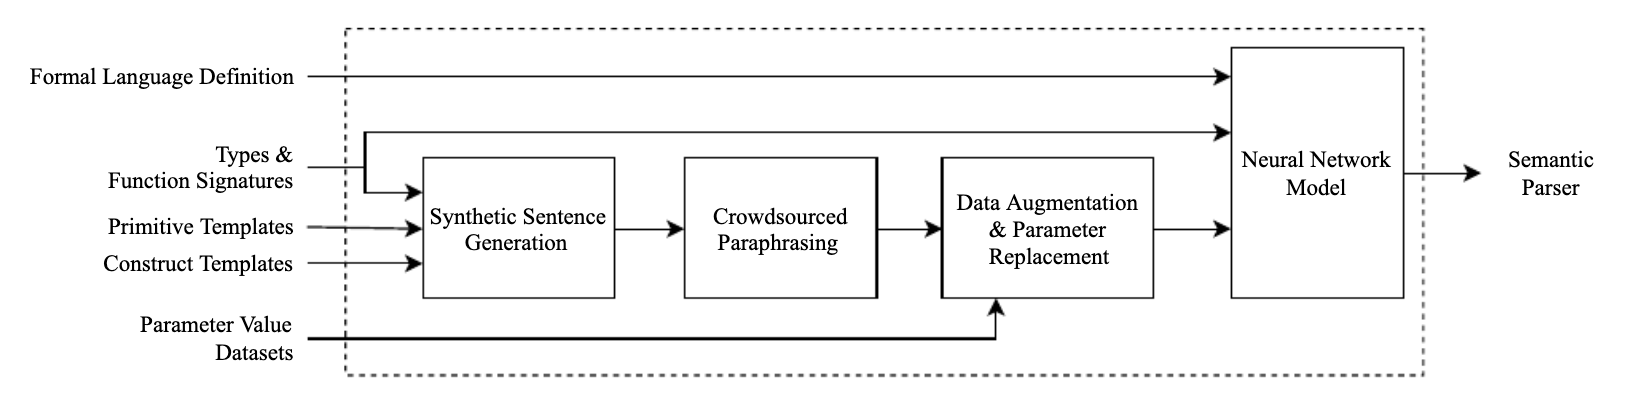
\includegraphics[width=\textwidth]{genie-vc.png}
    \caption[Overview of the Genie Semantic Parser Generator]{Overview of the Genie Semantic Parser Generator \citep{campagna2019genie}.}
    \label{fig:genie}
\end{figure}

A statistical distribution is the method typically used to generate synthetic data. This distribution is made for a set of samples from directly measured data. New values are created in the same format as the actual data. 

\cite{drechsler2010using} presented a procedure for synthetic dataset generation: "We define an order of the attributes that will be synthesised; values of the first attribute are synthesised by training the dataset synthesiser on the original dataset".

In the following sections, we will look at a series of dataset generation methodologies.

\section{Conditionial Distribution}
A conditional distribution is a distribution of values for one variable that exists when the values of other variables are specified. This distribution allows one to estimate the distribution of one's variable of interest under specific conditions.

The marginal probability (presented below) represents the probability of a single event occurring, independent of other events. On the other hand, a conditional probability represents the likelihood that an event occurs, given that another specific event has already occurred.

According to \cite{cond}, the aim of conditional distribution applied to dataset generation is that a random sample from the target conditional distribution can be obtained by the action of the conditional generator on a sample drawn from a reference distribution.

\section{Sampling from Independent marginals}
The Independent marginals method consists of sampling from the observed marginal distributions of each variable. Marginal probability is the name given to the probability of an event irrespective of the outcome of another variable \citep{indmargins}. 

The marginal distribution of a group of arbitrary variables is the probability distribution of the variables included in the group. It gives the likelihood of varied values of the variables in the group without reference to the values of the other variables. This distribution differs from a conditional distribution, which presents the probabilities considering the values of the other variables \citep{trumpler1953statistical}.

The independent marginals method approach has its advantages: it is computationally efficient. It possibly estimates marginal distributions for different variables in parallel. However, it does not capture statistical dependencies across variables. Therefore, the generated synthetic data may fail to capture the structure of the original data \citep{disclosure}.

\section{Bayesian network}
Bayesian networks are probabilistic graphical models. In these models, each node represents a random variable. The edges between the nodes represent probabilistic dependencies among the corresponding random variables. The graph structure and conditional probability distributions are inferred from the actual data \citep{baye}.

The learning process in Bayesian networks is comprised of two steps. The first one consists of learning a directed graph from the data. This graph expresses all the variables’ pairwise conditional dependencies (or lack thereof). The second step is estimating the conditional probability tables \citep{disclosure}.

The graph deduced from the actual data contains the conditional reliance among the variables. This graph also provides a visual representation of the variables’ relationships. By sampling from the inferred Bayesian network, we can generate synthetic data.

\section{Mixture of product of multinomials} %probably not gonna use this one
A multinomial experiment is a statistical experiment with a series of characteristics. The experiment consists of a set amount of repeatable trials. Each trial has a set number of outcomes and a constant probability for each outcome. These are independent, meaning that a previous trial does not influence future trials.

Any multivariate categorical data distribution can be expressed as a mixture of the product of multinomials (MPoM) \citep{dunson2009nonparametric}.

The multinomial model over term frequencies is defined in the Equation (\ref{eq:1}).

\begin{equation} \label{eq:1}
    P(\tilde{x}|\tilde{y}) =\frac{l!}{\prod _i x_{i}}\prod_{i=1}^{n}y_{i}^{x_{i}}
\end{equation}

where \(x_{i}\) is the number of times word \(i\) occurs, \(y_{i}\) is the mean parameter for word \(i\), and \(l=\sum _{i} x_{i}\) is the document length \citep{rennie2005mixtures}.

%We can view the multinomial as the following generative process. We have a hopper filled with balls. Each ball represents one of the n words and the hopper and balls are designed so that the chance of pulling a ball labeled word i is µi. Each hopper draw is a “word” event. Balls are replaced before the next draw. We tally word counts, but no not keep track of order information. The resulting set of counts is a “document” event.

Theoretical guarantees exist regarding the flexibility of this methodology to model any multivariate categorical data. However, this process can be very time-consuming in problems with large datasets.

%\section{Categorical latent Gaussian process}
%The categorical latent Gaussian process (CLGP) is a generative model for multivariate categorical data \cite{dunson2009nonparametric}. CLGP uses a lower dimensional continuous latent space and non-linear transformations for mapping the points in the latent space to probabilities (via softmax) for generating categorical values.

%Like BN and MPoM, CLGP is a fully generative Bayesian model, but has richer latent non-linear mappings that allows for representation of very complex full joint distributions. The inferred low-dimensional latent space in CLGP may be useful for data visualization and clustering.

%Inference for CLGP is considerably more complex than other models due to its non-conjugacy. An approximate Bayesian inference method such as variational Bayes (VB) is required.

%VB for CLGP requires several other approximations such as low-rank approximation for GPs as well as Monte Carlo integration. Hence, the inference for CLGP scales poorly with data size.

\section{Generative adversarial networks}
In the generative adversarial networks (GANs), two neural networks are trained jointly, competing. While the first network focuses on creating a realistic artificial dataset, the second tries to distinguish between natural and synthetic data from the first dataset. Due to the competition, each network pushes the other, leading to better results \citep{gans}. 

GANs have been successful in generating more complex data, being capable of producing synthetic images and text \citep{Mirza}. They are, however, incapable of producing categorical datasets. GANs cannot compute "gradients latent categorical variables for training vis backpropagation" - (in \cite{disclosure}). GANs do not require strict probabilistic models to perform their generation tasks. Therefore they are more flexible than the models previously mentioned. They can also deal with mixed data types.

When a GAN has many parameters, proper choice of multiple tuning ones (hyper-parameters) is difficult and time-consuming. GANs are also challenging to train. Solving the associated min-max optimization problem can be very unstable. This can, however, be circumvented if the variation Wasserstein GAN is applied \citep{gan}.

\begin{comment}
  
\section{Multiple imputation}
Multiple imputation is a method where several distinct possible datasets are created and the final dataset results from combining those datasets. This way, this approach is an optimal one to use in order to solve problems of missing data. 

The generation process starts with the creation of several copies of the dataset. These copies will have their missing values replaced by plausible imputed user values according to their original distribution.

The next set is the analysis of the created datasets. In this step, each dataset is analysed individually. This step is followed by combining these datasets in the proper output synthetical dataset.
\end{comment}

%The following sections are still transcribed and need to be rewritten and expanded
\section{Linear Regression}
Linear regression seeks to model the association between two variables by using a linear equation to the observed data. One variable is considered an explanatory variable, and the other is regarded as a dependent variable.

We can describe a linear regression line using the formula: \(Y = a + bX\). This formula's X is the explanatory variable, and Y is the dependent variable. The line slope is \textit{b}, and \textit{a} is the intercept (the value of \textit{y} when \textit{x = 0}).

To synthesise every attribute \(Y_{i}\) in a dataset, we learn the parameters of the regression model using the dataset with attributes in \(Y_{-i}\). We generate values for \(Y_{i}\) by sampling from a Gaussian distribution with constant variance and the mean as determined regression parameters.

\cite{regression} used linear regression to generate different datasets with the same estimates. This was developed for teaching purposes to demonstrate that different sets of regression data can give precisely the same estimated regression functions. 

\section{Decision Tree}
\cite{reiter2005using} proposed a generation technique that uses classification and regression tree. That author applied it to the generation of a partially synthetic dataset. The main components of a decision tree model are nodes and branches, and the most critical steps in building a model are splitting, stopping, and pruning \citep{song2015decision}.
\begin{figure}[t]
  \begin{center}
    \leavevmode
    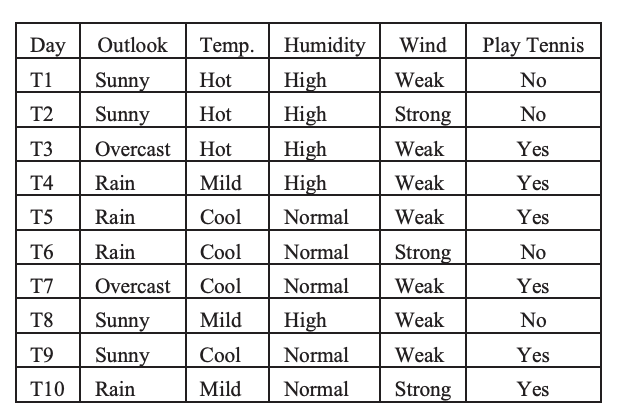
\includegraphics[width=0.5\textwidth]{dt_table.png}
    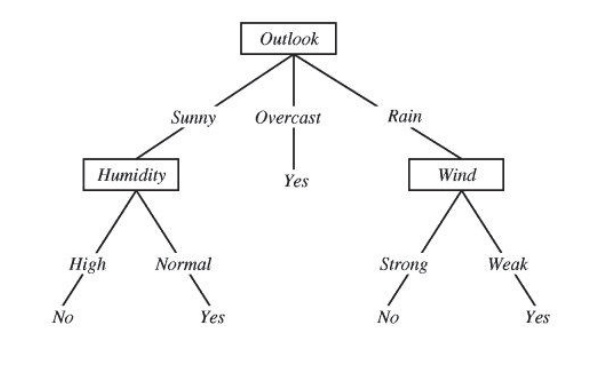
\includegraphics[width=0.5\textwidth]{dt_tree.png}
    \caption[Creation of a Decision Tree using a dataset]{Creation of a Decision Tree using a dataset [\cite{8226246}].}
    \label{fig:destree}
  \end{center}
\end{figure}

The process starts with building a decision tree using the values of the available attributes in the dataset \(Y-i\). To synthesise the value of an attribute \(Yi\) for a data point, we trace down the tree using the known attributes of the datapoint until reaching the leaf node. \cite{kirchner2004decision} applied this method to swine production and concluded that "the decision tree algorithm can detect relationships and patterns in real swine breeding datasets". Figure \ref{fig:destree} depicts a decision tree model created from a tabular dataset. An ML model was used to decide on a playing tennis binary problem. 


\section{Random Forecast}
Random Forest is a method introduced by \cite{breiman2001random}. As its name implies, a random forest consists of many individual decision trees that operate as a group. Each particular tree in the random forest releases a class prediction, and voting occurs for each class. The class with the most votes becomes our model’s prediction.

To synthesise values for a distinct point \(Yi\), a fixed number of decision trees on random samples of the training dataset \(Y-i\) are trained. The assemblage of results from the decision tree for a categorical attribute forms a multinomial distribution. For a continuous attribute, \cite{caiola2010random} propose using a kernel density estimator over the results from decision trees using sample values from the estimator.

\section{Neural Network}
Neural Networks are at the core of deep learning algorithms. They are inspired by the human brain, simulating how bodily neurons signal to one another \citep{abdi1999neural}.

Artificial neural networks (ANNs) incorporate node layers possessing an input layer, one or more hidden layers, and an output layer. Each node represents a neuron that connects to another and has an associated weight and target value (threshold). If the signal sent individual node is above the specified target value, that node is activated. Data is then sent to the next layer of the network.

Neural networks depend on training data to learn and improve accuracy over time. Nevertheless, once these learning algorithms are fine-tuned for precision, they are potent tools in computer science and artificial intelligence. This allows us to categorise and cluster data at a high rate.

%When looking at the dataset generation process, a neural network learns an abstract function mapping an input to the affiliated output as a data synthesiser. The output layer of a neural network incorporates K nodes (where K is the class classification problem). Each node represents the probability of the class being the model's output. We treat every attribute as a categorical variable. To synthesise the value of an attribute \(Yi\), we train a neural network using features in \(Yi-1\). We sample a value for attribute \(Yi\) using the output layer as a multinomial distribution.


\begin{comment}
  
\section{Evaluation}
One of the primary intents of enhancing a dataset generator is to increase the quality of the produced synthetic datasets. In order to evaluate the quality of a dataset, some methodologies are required.

The majority of evaluation functions use a scoring scheme. Let us suppose that D1 and D2 are datasets and \(E(x)\) is an evaluation function, and thus \(E(D1)\) and \(E(D2)\) generate some scores. If \(E(D1)>E(D2)\), we can expect that dataset D1 will yield better training/testing accuracy than D2.

\cite{dash1997feature} grouped evaluation functions into five categories: distance measures, information measures, dependency measures, consistency measures, and classifier error rate measures. Distance measures are the most popular and include separability, divergence, and discrimination measures. These measures were further analysed by \cite{4295518}. 

In the following sections, we will look at some evaluation approaches and points of interest when it comes to dataset evaluation.

\subsection{Distance Methods}
In this section, we summarize several distance measures for dataset evaluation. These measures are designed for feature evaluation, but they can be adopted for dataset evaluation. The goal of distance measurement is to calculate the distances among categories in a dataset.

\subsubsection{Euclidean distance}
The Euclidean distance between the two points \(p(p_{1}, p_{2}, p_{3}, …, p_{n})\) and \(q(q_{1}, q_{2}, q_{3}, …, q_{n})\) is defined as follows:

\begin{equation}
    d(p,q)=\sqrt{(p_{1}-q_{1})^2+(p_{2}-q_{2})^2+...+(p_{n}-q_{n})^2}
\end{equation}

Various equations can define Euclidean distance measure (EDM) for quantifying distance between two categories. One possible representation is:
\begin{equation}
    E(A,B)=d(c_{A},c_{B})-(r_{A}+r_{B})
\end{equation}

In this equation \(c_{A}\) and \(c_{B}\) are the center points of categories A and B. 
\(r_{A}\) and \(r_{B}\) are the radii of A and B. To calculate these values we can use the formula:
\begin{equation}
    r_{A}=\frac{1}{m}\sum_{i=1}^{m}d(c_{A},p_{i})
\end{equation}

Here \(m\) is the total number of points \(p_{i}\) and is a point in category A.

\subsubsection{Manhattan distance}
The Manhattan distance is similar to the Euclidian distance, but the distance between points \(p_{i}\) and \(q_{i}\) is calculated via a different equation.
\begin{equation}
    m(p,q)=\sum_{i=1}^{n}|p_{i}-q_{i}|
\end{equation}

Manhattan distance measure (MDM) can be defined as follows:
\begin{equation}
    M(A,B)=m(c_{A},c_{B})-(r_{A}+r_{B})
\end{equation}

\subsubsection{Hausdorff distance}
In mathematics, the Hausdorff distance, or Hausdorff metric, also called Pompeiu–Hausdorff distance \cite{birsan2005one}. It measures how far two subsets of a metric space are from each other. It turns the set of non-empty compact subsets of a metric space into a metric space in its own right. It is named after Felix Hausdorff and Dimitrie Pompeiu.

\begin{equation}
    \forall x_{1} \in A,D(x_{1},B) = min_{x_{2}\in B}\{d(x_{1},x_{2})\}
\end{equation}
\begin{equation}
    h(A,B) = max_{x_{1}\in A}\{D(x_{1},B)\}
\end{equation}
\begin{equation}
    H(A,B)=max\{h(A,B),h(B,A)\}
\end{equation}
These previous 3 equations display the needed steps for calculating the Hausdorff distance between set A and set B.

\(D(x_{1},B)\) is the distance between a point \(x_{1}\) in sets A and B, and \(d(x_{1},x_{2})\) means the distance between the two points \(x_{1}\) and \(x_{2}\). The directed function \(h(A, B)\) refers to the distance between set A and set B, and \(H(A, B)\) is also the distance between sets A and B. The Hausdorff Distance Measure (HDM) uses \(H(A, B)\) to calculate the distance among categories of a dataset.

\subsection{Comparison}
The measures presented before were analysed (alongside other metrics) by \cite{oh2011new}. They performed a series of analysis tests on 6 different datasets. The quality of this sets can be describe as follows: \(D_{1}>D_{2}>D_{3}>D_{4}>D_{5}>D_{6}\). The results can be seen in Fig. \ref{fig:dist_metrics}

\begin{figure}
  \begin{center}
    \leavevmode
    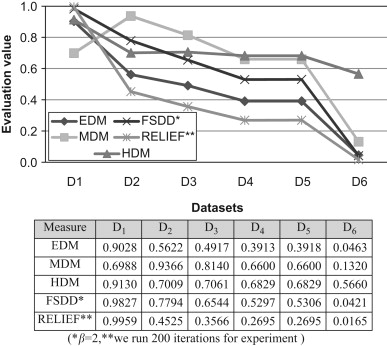
\includegraphics[width=0.7\textwidth]{metrics evaluation.jpg}
    \caption[Evaluation of distance metrics for dataset classification]{Evaluation of distance metrics for dataset classification \cite{oh2011new}}
    \label{fig:dist_metrics}
  \end{center}
\end{figure}
The relevant data to our study is the one related to the EDM (Euclidean distance measure), MDM (Manhattan distance measure) and HDM (Hausdorff Distance Measure). As we know that the datasets are numbered by highest quality to lowest quality, we can see that EDM proved more correct tham the others, with MDM having some problems with quantifying the quality of the 1st dataset and HDM performing the worst, being unable to identify major diferences betewenn the qualities if the datasets 2 to 5.

The other two methods displayed are used in feature selection.
\end{comment}

\section{Common dataset problems}
Other metrics exist that should be analysed when asserting the quality of a dataset. The usual suspects are overfitting, underfitting, missing data and data imbalances. In the following sections, we will look at these problems.

\subsection{Overfitting and Underfitting}
Overfitting might appear when a spurious pattern in the original dataset is captured and replicated with increasing frequency. This expands the amount of unnecessary random noise in the dataset. ML models trained with overfitted datasets are negatively impacted performance-wise. The random fluctuations of data are picked and learned as recurring moments \citep{over}.

Underfitting is the opposite of overfitting. It happens when the synthetic dataset does not capture enough relevant information from the original. Original metrics are not replicated, leading to a dataset with different distributions and metrics. ML models that used underfit datasets displayed poor performance ratios.

A graphical representation of overfitted and Underfitting can be found in Fig. \ref{fig:fitting}
\begin{figure}[!h]
  \begin{center}
    \leavevmode
    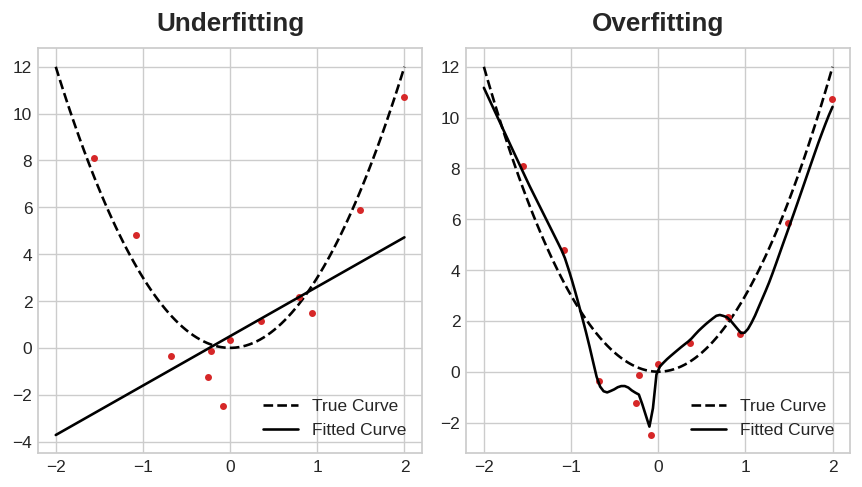
\includegraphics[width=0.7\textwidth]{underover.png}
    \caption[Underfitting and Overfitting]{Underfitting and Overfitting [\cite{holbrook}]}
    \label{fig:fitting}
  \end{center}
\end{figure}

\subsection{Missing Data}
Missing data is a problem that might also affect the quality of a dataset. It happens when no data value is stored for the variable in an observation. Missing data can significantly affect the conclusions drawn from the data.

Of course, when looking at data generation, two possible origins of missing data arise. It could be a bug of the generation software that can ultimately be corrected with due IT development. It could also be a problem in the original dataset used for the generation.

In actual datasets, missing data can occur due to a series of factors: data may be missing due to test design, failure in the observations or failure in recording observations.

\subsection{Data Imbalances}
Imbalanced data refers to datasets where the target class has an uneven distribution of observations. This is a problem in cases where small observations are relevant despite their minimal existence. For example, this can be seen in finance datasets for fraud detection, where the amount of fraud observations is very diminutive concerning the general data.

Mechanisms to prevent overfitting might increase the imbalance in the dataset as relevant data with minor occurrences could be considered noise.

\section{Data Evaluation}
For synthetic data to be considered valid, there needs to be evidence demonstrating the utility of that data. \cite{7waystodie} collected seven methods to evaluate the validity of synthetic data. Those methods are present in the following paragraphs.

The first method presented is structural similarity. Structural similarity indicates that the synthetic data should pass edit checks and have the same variable types and formats, variable names, metadata, file formats, table names and structure as real data does. The same methods used to analyse real data can be used on synthetic ones. 

General utility metrics assess general statistical parameters and model evaluation results. Using these metrics, it is also possible to assess the distinguishability between real and synthetic data. The synthetic data can be considered valid if an automated model cannot distinguish between real and synthetic data.

The utility of synthetic data can also be accessed through the replication of studies. Using this approach, we use an already-published study using the same dataset. We then replicate the results of that published study using the synthetic data. The data's validity depends on the success of the replication of results.

Letting domain experts examine the synthetic dataset and compare it to real data can also be a way to evaluate its quality. This evaluation is, however, subjective. 

Another evaluation metric is the Bias and Stability Assessment. This assessment consists of generating large quantities of synthetic datasets and calculating the general utility metrics on average. This evaluation is also valuable for evaluating the stability of the generation process.

Public available data could also be used in order to compare datasets. Synthetic datasets that reflect the same reality as publicly available real ones would be considered valid.

Comparison with Privacy-enhancing technologies is an option that can also be available. This assessment can help decision makers decide the relative strengths and weaknesses of particular PETs for providing data access.

\section{Conclusion}
In this section, we took a look at a series of methodologies and algorithms used in dataset generation. This analysis provides a series of metrics that can be helpful for the development phase.

However, bibliographic analysis of several dataset generation articles used different methods to generate datasets for other ends. We can see that each study develops its generation process per the final utilitarian purpose.

When looking at our generation, it should be noticed that application on the existing generator may not be optimal while these methodologies are helpful. The generator currently uses a configuration file that defines a series of restrictions and rules used in the synthesis. In our case, we can see that the generation process consists of an optimization problem to obey all limits while creating a dataset in the most optimal way possible. It could also be a simple generation with statistical distribution in mind. Everything depends on the configuration imputed by the user. 

Comparisons of applied improvements can be analyzed by looking at currently generated datasets generated at the end of this study using the same parameters. However, as the outcome of the generation depends on the user inputs, the system should allow for the generation of datasets of worse qualities.

We also presented ways to evaluate the quality of generated data. However, it should be noted that some of the presented evaluation methods will not be available in a purely synthetic generation.
\chapter{Problem and proposed solution} \label{chap:Problem}
The problem at hand is the extraction and inclusion of meta features in the Synthetic Dataset Generator SNOOKER generation process. This generator was initially produced by this study's second supervisor Leonardo Silva Ferreira. Simple generators face the problem of not generating realistic enough data or disclosing private information \citep{disclosure} when using a real dataset as a basis for the generation process.

The generator interface should allow users to select various meta features (explored in Chapter \ref{chap:mf}). Those meta features would be used in the generation process and be present in the final synthetic dataset, allowing for the creation of realistic datasets. 

When picking a generation algorithm, the first step will be to analyse the current generator and check its' methodology. If the current algorithm is not satisfiable enough, a new implementation must be made.

Some evaluation metrics should also be applied, and their results should be made available for the user at the end of the generation process.

\section{Snooker - An Overview}
\label{chap:Snooker}
Before analysing the problem, we should first look at the original generator, trying to understand its internal workings. SNOOKER was developed to bridge the availability gap for Helpdesk's datasets.

This section will present a general overview of the generator, talking about its leading technologies, features and the characteristics of its synthetically generated datasets.

\subsection{Technologies}

SNOOKER was developed using Python\footnote{\href{https://www.python.org/}{python.org}} and several of its libraries. Python is an interpreted, high-level programming language considered the standard for exploratory interactive and computation-driven scientific research \citep{5725235}. The user-generation interaction was handled by creating a graphical user interface (GUI).

The user interface of the generator was developed using PyQt\footnote{\href{https://pypi.org/project/PyQt5/}{pypi.org/project/PyQt5/}}. PyQt is a combination of Python bindings for cross-platform applications that combine all the strengths of Qt and Python \citep{siahaan2019postgresql}. This enables the development of GUI elements using Python Code. A print of the generator's GUI can be found in Figure \ref{fig:general_gui}.

The user can use the standard parameters in the presented interface or personalize the generation inputs as he wishes, fumbling with several interface options. After a short delay, a synthetical tabular dataset is generated after clicking the Generate button.

SNOOKER: A DataSet GeNeratOr fOr HelpdesK SERvices was developed using both technologies. A change in technologies in a study aiming to enhance the original generator would start the process from scratch, which would not be a viable option.

\begin{figure}[t]
  \begin{center}
    \leavevmode
    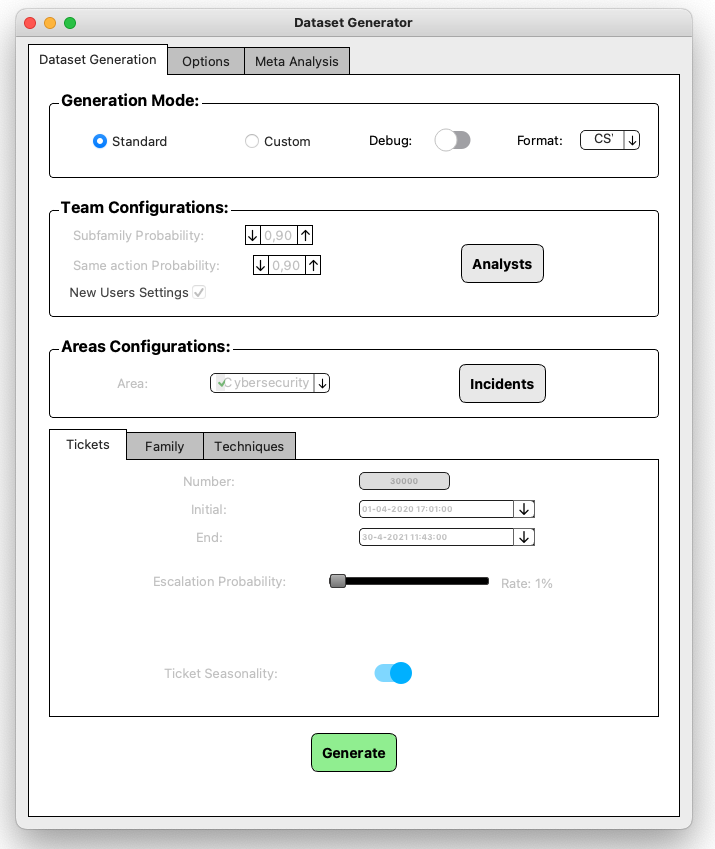
\includegraphics[width=0.6\textwidth]{general_gui.png}
    \caption{SNOOKER's User Interface}
    \label{fig:general_gui}
  \end{center}
\end{figure}

\subsection{Features}
The primary objective of SNOOKER was to enable synthetic helpdesk dataset generation. This dataset would take into account a series of features. The main features included in the generator are ticket management, team management and area management.

Tickets should be able to be customized (quantity, creation time, type, etc.), scheduled, treated (generation of appropriate treatment methods) and replicated if needed. 

The team management module handles the team's statistics (shift management, ticket percentages, etc.) and the singular team member information (general data connected to each member).

Lastly, the area management feature takes care of customizable incidents that might happen in each domain previously described.

It should also be noted that the generator uses as input not only the information provided by the user in the generator's UI but also data from a YAML configuration file.

\subsection{Synthetic Datasets}
SNOOKER's generated datasets contain much information commonly present in helpdesk datasets. While a complete representation of the synthetic dataset is not provided in this section, it can be examined in greater detail in Appendix \ref{ap3:snooker}.
%In this section, we will look at the final output from SNOOKER's generation process, explaining the information in each column of the dataset. The information regarding SNOOKER's outuputed dataset can be found on Appendix \ref{ap3:snooker}. 

\subsection{SNOOKER's generation process}
After receiving input from the previously mentioned configuration file, SNOOKER performs a series of tasks to fully generate each entry on the dataset. 

It starts the process by doing a simple Ticket Creation Task, where all the tickets are generated with simple data, and more complex data is added iteratively. Finally, the ticket family information is inserted in the final phase, where the family distribution over time is considered.

The following module in the generation is the Team Assignment. As its name suggests, this process is responsible for allocating teams and users available for each ticket. Shifts are considered for scheduling ticket-solving tasks by considering the team, work shift, and days not working for each team member.

The User Actions Creation module follows, providing the generator with valid actions (subtechniques) to solve each ticket problem based on its subfamily.

The following module is the Users Assignment. Each ticket is assigned a user and action by using the previously described modules in this process.

The fifth module takes care of Ticket replication tasks. This happens when a ticket is passed to more advanced teams. This event can be triggered when a ticket is created, when a set maximum number of tickets of that subfamily is detected, or when a set distance between the subfamily action and the user action exceeds the maximum distance defined in the interface.

Finally, the last module takes care of generating the Ticket Status. This status can either be 'closed' or 'transferred'. Transferred tickets also need to be replicated and passed to higher teams.

\section{Study Objectives}
Looking back at Chapter \ref{chap:intro} we should take a new look at the questions asked.

What selection of meta features should be calculated from the data in the synthetic dataset? In Chapter \ref{chap:mf}, we extracted several meta features that could be used. The final selection of meta features extracted from our datasets can be found in Chapter \ref{chap:class}.

What generation methods can we use? In Chapter \ref{chap:generation} we analysed a large group of algorithms that can be used to generate synthetic datasets. Of the available options, the one chosen and used later in Chapter \ref{chap:Integration}'s experiments was Conditional distribution. It is also the method used in SNOOKER's generation process.

Can we include specific values of meta features inside the generation process? This is touched on in the final development chapter of this study (Chapter \ref{chap:Integration}), where we study and discuss the possibility of including specific values of meta features inside the generation process.

What new additions can be added to the generator? Allied with the meta feature extraction module, we included a full-fledged meta feature extraction feature into the generator. More information regarding this feature can be seen in Chapter \ref{chap:class}. In Chapter \ref{chap:Conclusion} we also reference some future features that can be added to the application. Besides the inclusion of the new feature no other additions or changes were made to the original generator. 

The development of this study can be considered successful after fully answering the questions and furfilling the objectives presented in this section.

%If possible, the final product should be useful in creating ticket datasets and customisable types of datasets.

\section{Schedule}
Development of the final product went through several steps involving various tasks. A Gantt diagram was created to help with the planning. It can be found in figure \ref{fig:gantt}. 

\begin{figure}[h!]
    \begin{center}
      \leavevmode
      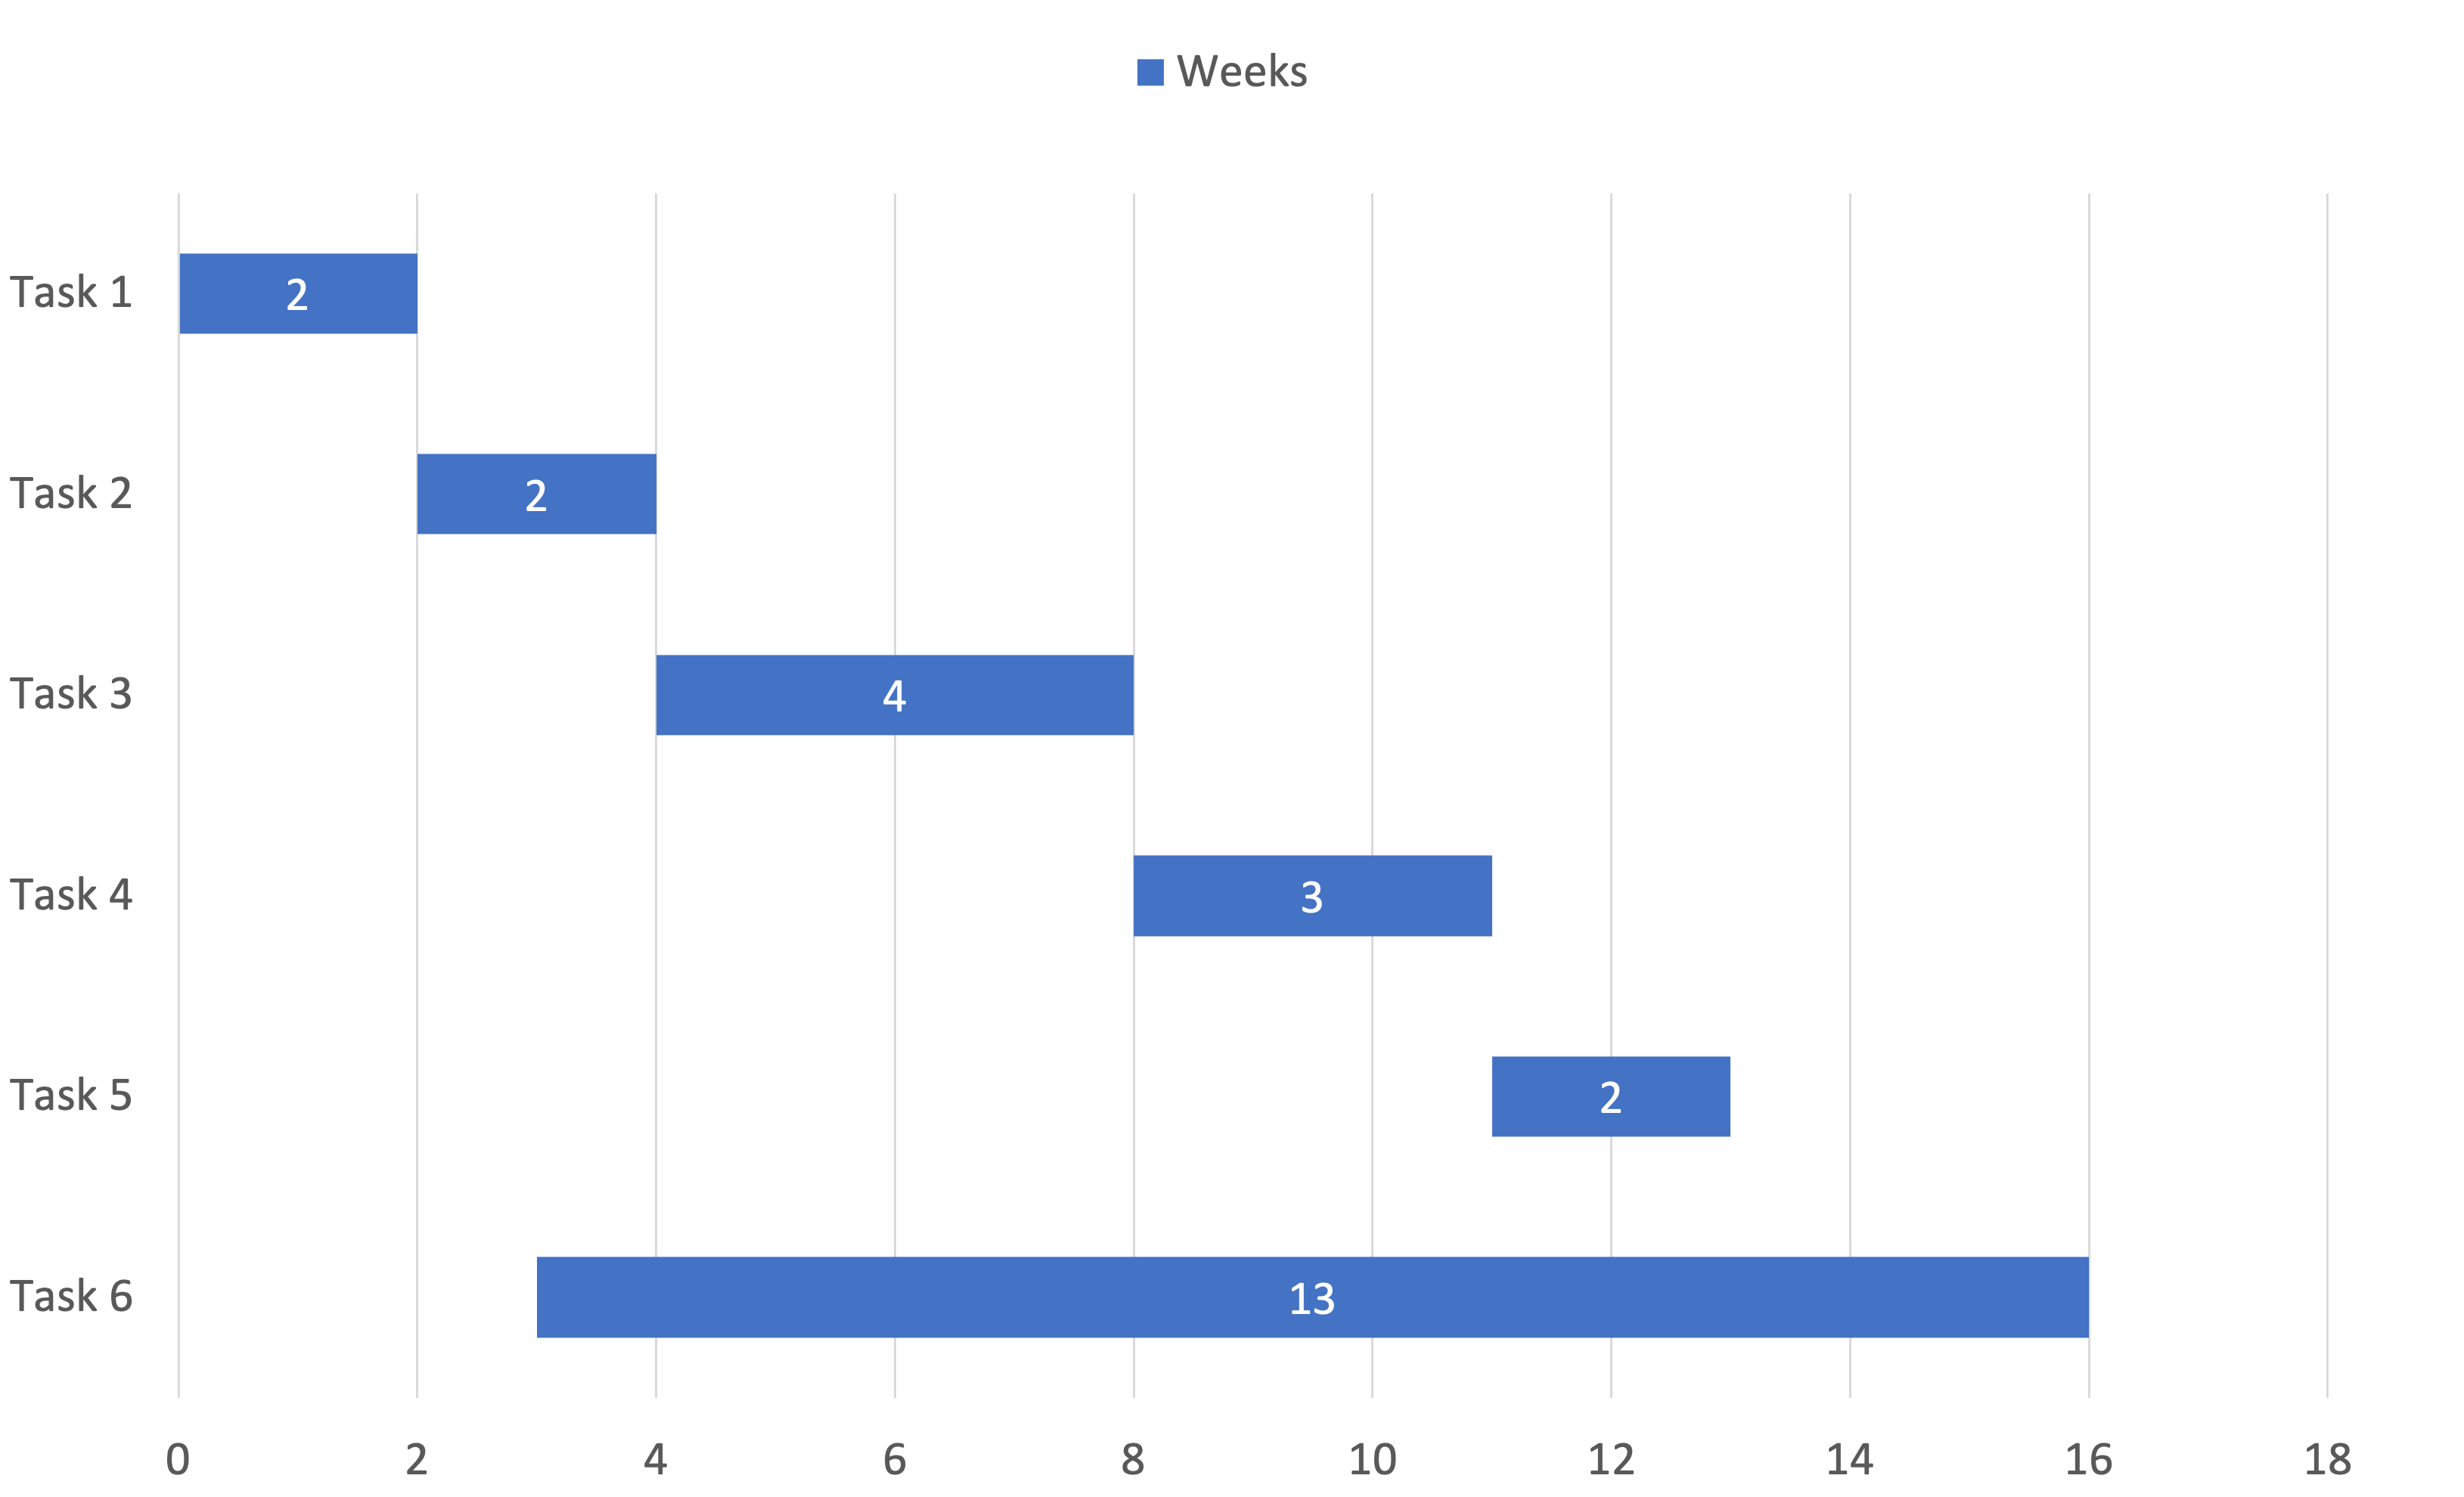
\includegraphics[width=1\textwidth]{gantt.png}
      \caption[Gantt diagram for the developed process]{Gantt diagram for the developed process}
      \label{fig:gantt}
    \end{center}
\end{figure}

Task 1 is the analysis of the current code. Task 2 is the implementation of improvements to the dataset generation process. Task 3 will explore the implementation of some meta feature selection. Task 4 regards quality validation of generated datasets. Task 5 will look at general improvements to the generator, namely in UI/UX. Finally, Task 6 is the writing of the dissertation and scientific paper.


\section{Risk Analysis}
The development of this project faced a series of risks. These risks were hindrances to the development process of the tasks previously depicted. We will now present a series of such potential threats. 

To start, we have to look at time constraints. The task at hand was challenging, and the short amount of time available to complete it made it impossible to deliver every single proposal task at the end.

Hardware limitations also impacted development. As some generation processes and meta feature calculations have high computational costs, an inefficient appliance delays the development, especially during trial-and-error periods. 

Another aspect that impacted development was the lack of know-how when dealing with data analysis and manipulation and the technologies used in the product.

\section{Projected vs Real work}
Ultimately the whole development part ended up not going as far as initially expected. We did not expect so many problems during the development of this project. Problems that ultimately left us still with much open to explore. The author idealised this study as an engineering problem with a core product that would be built upon. But ended up diving more into exploratory subjects, with no concrete answer regarding the inclusion of meta features in generation processes. While we know it is possible to do so, only small results were achieved and not enough to lead to valid proof of concept.

The real work ended up not following the scheduled plan. Analysis tasks took way more time than initially outlined. The quality assurance task became the meta feature extraction feature that took half of the available time to complete. The meta feature implementation (or integration as we now call it) was not fulfilled, being only theoretically explored.

On the other hand, the meta feature extraction tool serves as suitable proof of concept for the problem at hand. While the extraction in high dimensional datasets is still resource-intensive, this tool can perform each extraction task, given enough time.

Left behind were the practical meta feature inclusion module and the inclusion of enhancements to SNOOKER.
\chapter{Meta Feature Extraction}
\label{chap:class}

The first addition to SNOOKER: A DataSet GeNeratOr fOr HelpdesK SERvices was the inclusion of a meta feature extraction model. The objective was to allow users to extract meta features from the generated datasets, making it possible to extrapolate the quality of the synthetic data. It was also essential to enable meta-extraction of other datasets, making the product usable for meta-extraction tasks for datasets external to the generation.

Past development of the generator was made using Python. As the meta-extraction feature was idealized as an increment to the current product, it used the same language and foundation.

The evolution of this advancement proved quite troublesome; the development steps and the results are described in this chapter.

\section{Meta feature extraction}
Development started with manually coding the extraction of meta features from small (about 100 rows) synthetic datasets. A list of meta features to be included in the analysis was made, considering the information acquired in Chapter \ref{chap:mf}.

Testing started with the simple meta feature analysis of a dataset. As the generator creates synthetic datasets in a .csv (Comma-separated values) format, a way to analyse such data was necessary. One major issue for would-be statistical Python programmers in the past has been the lack of libraries implementing standard models and a cohesive framework for specifying models. Pandas\footnote{\href{https://pandas.pydata.org/}{pandas.pydata.org}} is a Python library of rich data structures and tools for working with structured data sets. It is commonly used in statistics, finance, social sciences, and many other fields \citep{mckinney2011pandas}. It intends to close the gap in the richness of available data analysis tools between Python, general-purpose systems and scientific computing language, and the numerous domain-specific statistical computing platforms and database languages. Pandas was therefore used.

General meta feature analysis was relatively simple to implement due to being directly observable from the dataset, representing basic information and being the most explicit set in terms of computation cost. Problems arrived when looking at the analysis of statistical meta features. 

The development of models to analyse every statistical meta feature was slow. Continuing down that path would limit the scope of the work given the existing time frame and delivery dates. The solutions available were to limit the number of analysed meta features (extracting only a hand full per family) or to rely on external tools to perform that same task. The latter option was chosen. After consideration, the Python library Python Meta Feature Extractor (pyfme\footnote{\href{https://pymfe.readthedocs.io/en/latest/index.html}{pymfe.readthedocs.io}}) was selected and used to perform meta feature extraction tasks.

The pymfe library provides a comprehensive set of meta features implemented in python. According to the library developers, the package brings cutting-edge meta features, following recent literature proposals. The pymfe architecture was idealised to systematically make the extraction, which can produce a robust set of meta features. The review performed by \cite{alcobacca2020mfe} agreed with our decision and proved a suitable validator. As such, development moved forth using this library.

Pymfe can extract several families of meta features from a dataset. Those families are depicted in the following list, with tables describing every family's meta feature presented in Appendix \ref{ap1:pymfe_mf}.
\begin{itemize}
  \item \textbf{General}: General information related to the dataset, also known as simple measures, such as the number of instances, attributes and classes (Table \ref{tab:pymfe-general-mf}).
  \item \textbf{Statistical}: Standard statistical measures to describe the numerical properties of data distribution (Table \ref{tab:pymfe-statistical-mf}).
  \item \textbf{Information-theoretic}: Particularly appropriate to describe discrete (categorical) attributes and their relationship with the classes (Table \ref{tab:pymfe-it-mf}).
  \item \textbf{Model-based}: Measures designed to extract characteristics from simple machine learning models (Teable \ref{tab:pymfe-mb-mf}).
  \item \textbf{Landmarking}: Performance of simple and efficient learning algorithms (Table \ref{tab:pymfe-landmarking-mf}).
  \item \textbf{Relative Landmarking}: Relative performance of simple and efficient learning algorithms.
  \item \textbf{Subsampling Landmarking}: Performance of simple and efficient learning algorithms from a subsample of the dataset.
  \item \textbf{Clustering}: Clustering measures extract information about dataset based on external validation indexes (Table \ref{tab:pymfe-clustering-mf}).
  \item \textbf{Concept}: Estimate the variability of class labels among examples and the examples density (Table \ref{tab:pymfe-concept-mf}).
  \item \textbf{Itemset}: Compute the correlation between binary attributes (Table \ref{tab:pymfe-itemset-mf}).
  \item \textbf{Complexity}: Estimate the difficulty in separating the data points into their expected classes (Table \ref{tab:pymfe-complexity-mf}).
\end{itemize}

The vast amount of families and collections of meta features inside those families proved more than enough to use in our meta-extraction model. Some limitations were, however, applied. Pandas is unable to analyse datasets with missing data. Meta features that use missing data as a parameter had to be left out.

Right in the start, the library requires the definition and extraction of the first column from the dataset to analyse CSV data. The definition of the column name can be surpassed using pandas' ability to read information from CSV data. The program can automatically grab the first column from a dataset. The generator already creates an expendable 'ID' column in its first position, which can be consumed without affecting the meta feature analysis result. However, this does not apply to other possible datasets, forcing users to edit datasets not generated by SNOOKER to get valid results. The snippet \ref{lst:pandas} shows an example of code used to read the CSV file while consuming the first column.

\par\noindent\rule{\textwidth}{0.4pt}
\begin{lstlisting}[language=Python, caption=Importing the csv dataset with ID column, label={lst:pandas}]
  df = pd.read_csv(path, sep=";", index_col=False)
  X, y = df.drop(df.columns[0], axis=1), df[df.columns[0]]
\end{lstlisting}
\par\noindent\rule{\textwidth}{0.4pt}

Another simple limitation was defining a sep for the CSV data. In the case of SNOOKER, CSV is generated using semi-colons, which was the used value for steps.

The meta-extraction feature was intended as the main addition to SNOOKER. It needed to be integrated into the generator's interface, making it possible to be accessible to users in a simple way. The development of the interface will be tackled in the next section.

Each meta feature family selected outputs a file at the end of the analysis. This file contains the path to the analysed dataset, the results of each meta feature inside that family and the time it took to perform that meta feature extraction. A transcription of an actual output file from a meta feature extraction analysis can be found in Appendix \ref{ap2:meta_files}.

\section{Interface}
The Meta Feature Extraction Module was always idealized as an increment made to SNOOKER during this study. As such, it needed a user interface to allow user-module interaction. An interface was created and appended to the generator's frontend. As seen in Chapter \ref{chap:Problem}, SNOOKER's interface was developed using PyQt, which meant that this interface had to be developed using the same technology.

"Python is probably the easiest to learn and nicest scripting language in widespread use, and Qt is probably the best library for developing GUI applications. The combination of Python and Qt, "PyQt", makes it possible to develop applications on any supported platform and run them unchanged on all supported platforms" (quoted from \cite{summerfield2007rapid}).

%PyQt5 is the latest version of a GUI widgets toolkit developed by Riverbank Computing. It is a Python interface for Qt, one of the most powerful, and popular cross-platform GUI library. PyQt5 is a blend of Python programming language and the Qt library.

The interface went through an idealization period, and the concept and objectives changed. Originally the interface was supposed to have a button that would trigger a file selection. This selection would generate a series of rows containing that file's column names. Next to each column name, we would have a toggle feature to select columns to use in the calculations. It would also be accompanied by a dropdown containing options to select the data type in that column (Numeral, Text, Date, etc.). The concept for the original interface can be found in Figure \ref{fig:class_original_interface}. 

\begin{figure}[t]
  \begin{center}
    \leavevmode
    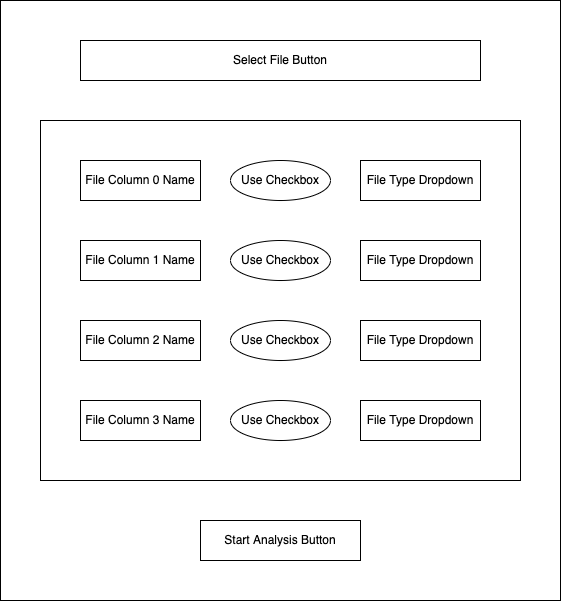
\includegraphics[width=0.5\textwidth]{original_idea.png}
    \caption{Original idealization of meta-extraction feature interface}
    \label{fig:class_original_interface}
  \end{center}
\end{figure}

The meta feature calculations were coded by hand, using a series of measures requiring user input on each column's data type. The system could not distinguish between categorical and numeric features, creating error breaks in the analysis. Although implementation started, it was quickly dropped, and no visual record was kept of its development.

When moving to the pymfe library, the interface changed to focus on more relevant features, the selection of meta features. The current implementation keeps the file selection button. Still, it forgoes the column toggle and data type selection, using a simple toggle of meta feature families. Figure \ref{fig:class_interface_2} depicts the final interface. 



\begin{figure}[!h]
  \begin{center}
    \leavevmode
    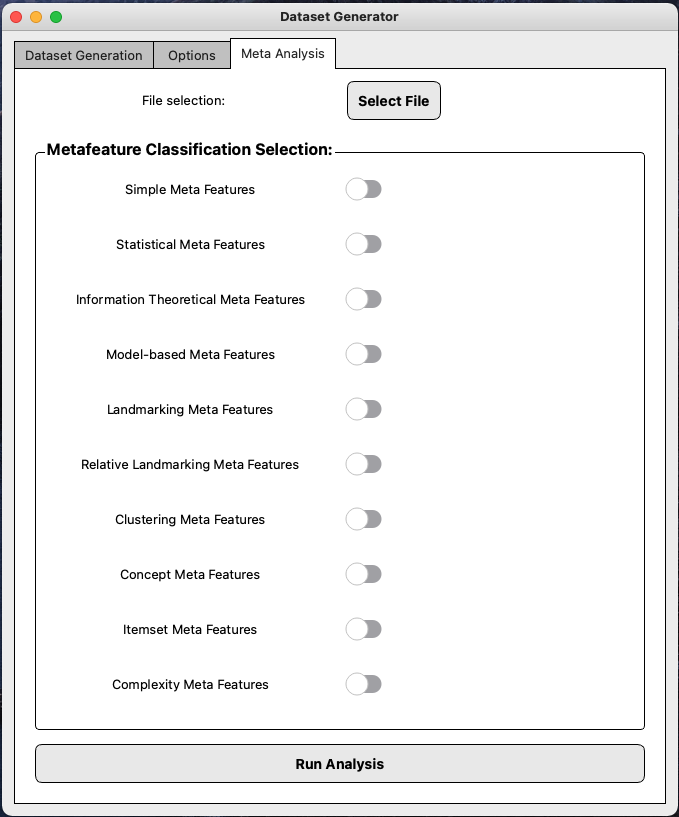
\includegraphics[width=0.6\textwidth]{interface_class_2.png}
    \caption{Meta Feature Extraction feature interface }
    \label{fig:class_interface_2}
  \end{center}
\end{figure}

\section{Library Limitations}
Opting to use the pymfe library proved to be the right choice, as it propelled the development of a large number of steps. It was possible to classify datasets with a giant gallery of meta features. However, some limitations were accompanied by the library. 

One such limitation was quickly found: the time needed to perform meta feature extraction analysis. While small datasets took only a few minutes to analyse, as the size of the dataset increased, so did the time the analysis took to finish. Several tests were made and data extracted to see what families of meta features were causing the output delay. That data can be found in Table \ref{tab:analysis_time}. It should be noted that way more tests were made during the development of this study. Nonetheless, results were sometimes incomplete and/or used datasets with different amounts of columns. The datasets chosen to perform this first analysis were all generated by SNOOKER.

\begin{table}[h!]
  \centering
  \caption{Testing made on the meta-extraction feature, using several datasets. }
  \setlength{\tabcolsep}{8pt}
    \renewcommand{\arraystretch}{1.2}
      \begin{tabular}{llllll}
        \hline
        Meta Feature family     & DS1       & DS2       & DS3       & DS4       & DS5 \\ \hline
        Simple                  & 2.21s     & 3.25s     & 6.27s     & 11.90s    & 32.70s\\
        Statistical             & 28:16 min & 17:06 min & 12.22 min & >2h       & 51:31 min\\
        Information Theoretical & 24.82s    & 21.9s     & 45.72s    & 43.55s    & 1:26 min\\
        Model-based             & 4.47s     & 1:15 min  & 25:42 min & >2h       & >2h \\
        Landmarking             & <1s       & 2.69s     & 5.34s     & 23.07 s   & 38.73s \\
        Relative Landmarking    & 6.25s     & 2.19s     & 5.23s     & 17:06 min & >2h \\
        Clustering              & 3:13 min  & 4:29 min  & 13:19 min & 45:23min  & >2h \\
        Concept                 & 8.52s     & 29.02s    & 58.32s    & 52.15s    & 57.46s\\
        Itemset                 & 5.14 min  & 10:38 min & 23:57 min & >2h       & >2h\\
        Complexity              & >4h       & >4h       & >4h       & >4h       & >4h \\\hline
  \end{tabular}
  \label{tab:analysis_time}
\end{table}

DS1, DS2, DS3 and DS4 were SNOOKER-generated datasets with 1000, 2000, 3000, 4000 and 5000 entries, respectively. Some outliers can be found on datasets with more entries where certain calculations took way more time than the rest. Many outliers can be attributed to hardware limitations. Overheating and memory problems were faced when leaving the meta-extractor module running for hours. However, we can see that statistical analysis took more time than any other analysis. Complexity analysis was also incapable of reaching any result, even having double the available time limit to perform said analysis. Initially, the sentiment was that hardware limitations were accountable for these analysis times. Yet, when testing the meta-extraction feature on a much more powerful machine, the end result times were similar to those achieved locally. It could then be concluded that the statistical and complexity times problem was not the computational power. 

Regular analysis was kept running for a maximum amount of 2 hours per meta family. However, complexity analysis took way more time from the beginning. We tried to see how far we could go on their research, making 2 tests with 2 different datasets with a time limit of 12 hours. Both these tests were unable to lead to results. We then tried using datasets with a low number of entries. This analysis's result is displayed in Table \ref{tab:small_analysis_time}. We used 5 SNOOKER-generated datasets with 100, 200, 300, 400 and 500 entries. We compared the time it took to perform a statistical analysis (the second most time-consuming analysis) to the time taken by complexity calculations. On that same table, we also have a Ratio row. This ratio indicates the $ComplexityTime/StatisticalTime$ relation.
\begin{table}[b]
  \centering
  \caption{Complexity and Statistical runtimes on small datasets}
  \setlength{\tabcolsep}{8pt}
    \renewcommand{\arraystretch}{1.2}
      \begin{tabular}{llllll}
        \hline
        Entries     & 100       & 200       & 300       & 400       & 500 \\ \hline
        Statistical & 1.5s      & 10.60s    & 38.52s    & 1:25 min  & 2:55 min \\
        Complexity  & 53.62s    & 5:53 min  & 17:46 min & 40:17 min  & 1:24:53 h \\\hline\hline
        Ratio       & 35.75     & 33.30     & 27.67     & 28.44     & 29.01\\\hline
  \end{tabular}
  \label{tab:small_analysis_time}
\end{table}

From the analysis, we could conclude that Complexity analysis took way too much time to complete compared to other meta-calculations. Further investigation of these meta features was dropped as time constraints made their study impossible to pursue. The option to analyse them is still present in the current product. However, due to the limitations mentioned earlier, its use is not recommended on local machines.

While Complexity Meta-Analysis was dropped from further development. The same could not apply to Statistical Meta Features as their values are some of the most important we could extract from a dataset. So what if we could remove some meta features from the module? The idea was to test each statistical meta feature extraction. We would save each analysis's time and remove more time-consuming meta features, making the calculation faster. 

We used the previously used SNOOKER-generated datasets to get the statistical analysis times. However, it soon became obvious that it would take too much time. Complete statistical analysis of SD1 took more than 15 hours to complete (the output of this analysis can be seen in Appendix \ref{appendix:statistical}). We decided to use a series of smaller, publicly available datasets\footnote{\href{https://perso.telecom-paristech.fr/eagan/class/igr204/datasets}{perso.telecom-paristech.fr}}. Several other datasets were also used in the analysis, but as dataset dimensionality grew, so did time required to analyse all 19 meta features plus the full analysis. Runtime of each analysis is presented in Table \ref{tab:stat_analysis_time}.

\begin{table}[t!]
  \centering
  \caption{Statistical meta analysis duration}
  \setlength{\tabcolsep}{8pt}
    \renewcommand{\arraystretch}{1.2}
      \begin{tabular}{llllll}
        \hline
        Meta Feature  & SD1   & cars & cereal & CausesOfDeath\_France\_2001-2008 \\ \hline
        can\_cor      & 26:32 min &50.97s & 0.48s & 13:07 min \\
        cor & 27:16 min & 52.99s & 0.46s & 12:31 min\\
        cov & 25:29 min & 52.40s & 0.46s & 12:25 min \\
        eigenvalues & 31:03 min & 52.54s & 0.47s & 11:25 min \\
        g\_mean & 25:42 min & 52.55s & 0.46s & 11:37 min \\
        gravity & 26:54 min & 52.16s & 0.45s & 11:38 min \\
        h\_mean & 25:32 min & 52.11s & 0.45s & 11:38 min \\
        iq\_range & 27:45 min & 1:44 min & 0.46s & 11:31 min\\
        kurtosis & 26:54 min & 1:07 min & 0.51s & 11:36 min\\
        lh\_trace & 26:04 min & 54.09s & 0.45s & 11:34 min\\
        mad & 28:52 min & 52.51s & 0.45s& 11:34 min\\
        max & 26:29 min & 52.51s & 0.44s & 11:34 min\\
        mean & 26:56 min & 51.85s & 0.44s & 11:36 min\\
        median & 27:36 min & 51.88s & 0.44s & 11:33 min\\
        min & 26:31 min & 51.57s & 0.45s & 11:31 min\\
        nr\_cor\_attr & 47:58 min & 51.03s & 0.44s & 11:29 min\\
        nr\_disc & 27:54 min & 50.70s & 0.44s & 11:30 min\\
        nr\_norm & 27:40 min & 51.09s & 0.45s & 11:29 min \\
        nr\_outliers & 24:35 min & 50.99s & 0.44s & 11:33 min\\
        p\_trace & 24:35 min& 50.77s & 0.44a& 11:35 min\\
        range & 35:49 min & 51.02s & 0.44s & 11:35 min\\
        roy\_root & 26:51 min& 52.16s & 0.44s & 11:36 min\\
        sd & 26:14 min & 51.04s & 0.45s & 11:40 min\\
        sd\_ratio & 27:26 min & 50.71s & 0.45s & 11:37 min\\
        skewness & 24:42 min & 50.95s & 0.49s & 12:05 min\\
        sparsity & 27:49 min & 50.67s & 0.42s & 11:24 min \\
        t\_mean & 25:17 min & 50.95s & 0.43s & 11:13 min\\
        var & 24:23 min & 51.76s & 0.42s & 11:10 min\\
        w\_lambda & 23:56 min & 50.65s & 0.43s & 11:08 min\\
        FULL ANALYSIS & 28:16 min& 51.44s & 62.65s & 11:25 min\\
        \hline
  \end{tabular}
  \label{tab:stat_analysis_time}
\end{table}

The outcome of this analysis was unexpected. Even with some calculations taking more time, the differences are predominantly negligible. In fact, the last row shows that the library takes roughly the same time to perform a complete analysis as it does on every individual meta-extraction computation. With this result, proceeding with analysing more enormous datasets proved unnecessary.

Further exploration of the pymfe library proved that improving the calculations it made would be a daunting task. Pymfe was developed by \citet*{alcobacca2020mfe} the leading experts in the field regarding meta analysis. A full review of the library found on kandii\footnote{\href{https://kandi.openweaver.com/python/ealcobaca/pymfe}{https://kandi.openweaver.com/} - kandi is a code and library review website} also showed that the library is of the highest quality. Its most significant flaws were its high code complexity (9614 lines of code, 461 functions and 56 files) and lack of current releases (it had no major release in the last 12 months). As code complexity directly impacts the maintainability of the code, trying to influence its results would require more time and resources than what was available. We were left with no choice but to accept the high wait times when researching some meta feature families.

While abandoning problematic families could alleviate the problem, it would not solve it. Even general meta feature extraction could take a long time to complete, given a large enough dataset. In fact, even problematic familes can achieve results in smaller datasets. Ultimately, looking at the tool as a product, we find it more beneficial to leave the choice up to the end user than to remove it outright.

The meta-extraction module was considered finished with the decision that no further improvements could be made.

\section{Conclusion}
In this chapter, we took a look at the development process for the meta feature extraction module, created as an addition to SNOOKER. We started the chapter by displaying our path until we arrived at an agreeable solution for the meta feature extraction problem. After trying to make all the calculations ourselves, we used the pymfe library to accelerate the process, adding an enormous amount of meta features to the analysis pool.

In the second section, we explore the development of the module's interface, developed using PyQt5. The interface went through a series of alterations and experimentations until we arrived at the current presentable stage.

Lastly, we did some experiments on the final product, identifying problems and finding a way to correct them. Unfortunately, no way to solve the detected problems was found.

Ultimately the Meta-extraction feature ended up going further than what was initially planned. The original concept was to develop this meta-analysis from scratch, getting only some examples from each family. Ultimately, pyfme allowed us not to get some meta feature results but tens of results per analysis. On the matter of optimization, the feature does, however, underperform.
\chapter{Meta Feature Integration}
\label{chap:Integration}

In the following chapter, we will explore the conclusive part of this dissertation: the study and methodology for including meta features in the generation process.

Synthetic datasets with specific meta features can help generate better datasets. For starters, randomly generated datasets cannot ensure a good distribution of meta features, leaving sparsely populated areas inside the "meta feature space". Secondly, generating datasets with specific values of meta features allows more controlled experiments that might lead to conclusions about the usefulness of particular meta features \citep{reif2012dataset}.

However, using the current generator and applying meta feature forcing proved too tacky and time-consuming. As seen in Chapter \ref{chap:Problem} Section \ref{chap:Snooker}, SNOOKER generates datasets with helpdesk ticket solving; the final dataset contains a lot of information (regarding ticket generation, team management, and scheduling). Every entry was too large and had too many variables to correctly influence globally. Dimensionality was, therefore, a problem. As the dataset's final dataset could be understood as a kind of DATALAKE dataset, what was decided was to study the insertion of a meta feature on one of those modules.

We developed some experiments using a subset of a dataset output from SNOOKER, using columns related to ticket generation, reducing the dimensionality of the dataset. Experimentation was simple and purely exploratory. A more prominent focus was taken on exploring possible meta features to be included and methods that would facilitate that inclusion.

What was left was some of the previously referred meta families. Then, select a set of meta features, study their characteristics and see how to better include them in the generation process. While a collection of meta features is presented below, it was unknown if their inclusion would be considered helpful at the moment of selection. Each meta feature was analysed on its individuality, taking into no account the result from a combination of forcing these meta features in the same generation process.

\section{General}
General meta features are the simplest ones to force onto a dataset, as they are closely connected to the main parameters and characteristics of the generated synthetic dataset. One aspect associated with the general meta feature family is dataset dimensionality.

Dimensionality in statistics refers to how many attributes a dataset contains. In the case of tabular datasets, this data could be represented in a spreadsheet, with one column representing each dimension. 

High-dimensional data relates to a dataset where the number of Attributes (or columns) is more significant than the number of Instances (or lines). For example, we can regard a dataset with twenty attributes and merely seven instances as a high-dimensional dataset. As we can witness, the number of features is larger than the number of observations. High dimensionality datasets are challenging to address. It is also problematic to categorise such high dimension data. High dimensionality also carries some redundant features, ushering in data losses \citep{ray2021various}.

It should be mentioned that even if a dataset has many attributes if the number of instances surpasses that point, it cannot be regarded as a high dimensionality dataset \citep{ziegel2003elements}.

We will now look at one meta feature connected with dimensionality - \textit{attr\_to\_inst}. This meta feature represents the ratio between the number of instances and attributes in the dataset. Let's now see if it is possible to force a value of this meta feature onto the generation process and if this inclusion is valuable.

Regarding the inclusion of a specific general meta feature value to a synthetic dataset, how can we force a particular value of \textit{attr\_to\_inst} during generation? To start it off, let's take a look at the needed calculations. Let's use $\alpha$ to represent the number of attributes and \textit{n} to represent the number of instances. The formula to calculate \textit{attr\_to\_inst} meta feature can be seen in Equation \ref{eq:attrtoinst}.

\begin{equation}
  \label{eq:attrtoinst}
  attr\_to\_inst=\frac{\alpha}{n}
\end{equation}

Now to proceed, some basic rules were applied. Both $\alpha$ and \textit{n} need to be natural integer numbers more significant than zero. We also decided that adding or removing entries was fair game. However, doing the same for the number of columns could remove information essential to the dataset. Some rules were added to guarantee the preservation of the original dataset's attributes. \ref{eq:alpha} is one of such rules.

\begin{equation}
  \label{eq:alpha}
  \alpha = O + \delta
\end{equation}

Where \textit{O} is the original dataset's column count, and $\delta$ represents the number of added columns to the synthetic dataset.

Two more conditions should be added to certify that no error occurs during the calculations. Those conditions are presented in Equations \ref{eq:deltab0} and \ref{eq:b1}.

\begin{equation}
  \label{eq:deltab0}
  \delta \geq 0
\end{equation}

\begin{equation}
  \label{eq:b1}
  \alpha, O, n \geq 1
\end{equation}

And Equation \ref{eq:positive} one guarantees that all values are positive integers.

\begin{equation}
  \label{eq:positive}
  \alpha, n, O, \delta \in \mathbb{I}
\end{equation}

Having all the needed formulas, we can concur that we need to solve an optimization problem to achieve a desirable dimensionality value. Using the equations presented in \ref{eq:condi} that come from simplifying the previously shown ones, we should be able to solve the optimization problem that leads to the desired result.

\begin{equation}
  \label{eq:condi}
  \begin{aligned}
      D = \frac{\alpha}{n} &
      \\\alpha \geq O &
      \\\alpha, n, O \geq 1 &
      \\\alpha, n, O \in \mathbb{I}
  \end{aligned}
\end{equation}

Knowing our \textit{attr\_to\_inst} value (represented in the previous equation by \textit{D}), we can solve the optimization problem by getting the values of $\alpha$ and \textit{n} that are a solution to the problem. According to the results, the generator can tweak its parameters to grow vertically and/or horizontally.

Now that we solved the forced inclusion of a set \textit{attr\_to\_inst} value, let's now see how sound is this inclusion.

The dataset could expand both vertically and horizontally. Vertical expansion is already used in synthetic dataset generation. It would simply change the number of entries to the dataset. Definition of the number of entries is an essential feature required in dataset generation, typically using user input to get this value. On the other hand, horizontal growth is a more particular feature that isn't generally available on generators using already existing datasets as a basis. However, a critique should be made of the final synthetic dataset. How valuable would the extra randomly generated data actually be? Especially when looking at machine learning, adding useless information would actually be prejudicial. 

We concur that the dimensionality of a dataset should be extracted. However, forcing a set value for a dimensionality-related meta feature (like \textit{attr\_to\_inst}) is not helpful in dataset generation.

\section{Statistical}
Assembling datasets with set values for statistical meta features would facilitate the creation of more diverse and valid datasets. These would have different characteristics, all using the same original dataset. Indicating that there is value in diving into forcing some of these meta features into a synthetic dataset. In this section, we will look at skewness and kurtosis, seeing how their inclusion would change the dataset and displaying a way to force them into the generation process.

\subsection{Skewness}
In probability theory and statistics, skewness is a measure of the asymmetry of the probability distribution of a real-valued random variable about its mean \citep{dean2018descriptive}. The skewness value can be positive, zero, negative, or undefined. It describes the distribution shape of the measured values in terms of symmetry \citep{rivolli2019characterizing}. 

Figure \ref{fig:skewness} shows a visual representation of skewness. In this figure, the first graphic depicts a left skewness, informing us that the mean of the values is smaller than the median, which is smaller than the mode. The central graph illustrates a symmetrical normal, where the mean, median and mode share the same value. Finally, the right figure depicts a skewed right graph. In this type of skewness, the mean is greater than the medium, that is, greater than the mode.

\begin{figure}[ht]
  \begin{center}
    \leavevmode
    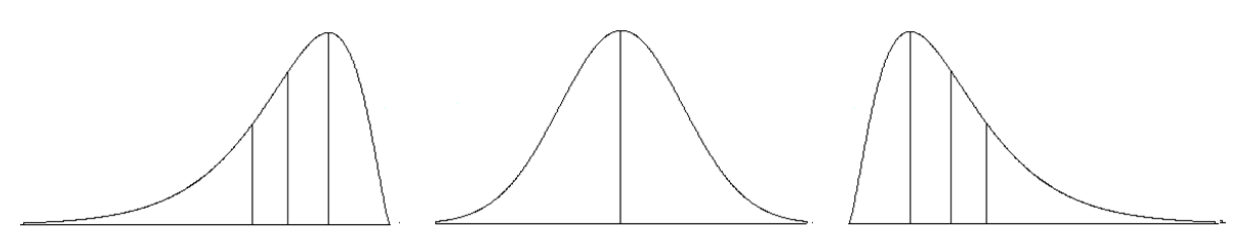
\includegraphics[width=1\textwidth]{skewness.png}
    \caption[Visual representation of skewness]{Visual representation of skewness. Removed from \cite{doi:10.1080/10691898.2011.11889611}}
    \label{fig:skewness}
  \end{center}
\end{figure}

The skewness of attributes is calculated through the Equation \ref{eq:skew}:

\begin{equation}
  \label{eq:skew}
  skewness_x=\frac{m_3}{sd_x^3}
\end{equation}

Where $sd_x^3$ and $m_3$ are extracted from the formulas \ref{eq:skew1} and \ref{eq:mj}.

\begin{equation}
  \label{eq:skew1}
  sd_x^3=\sqrt{\frac{\sum_{i=1}^{n}(x_i - \bar{x})^2}{n-1}}
\end{equation} 

\begin{equation}
  m_j=\frac{1}{n}\sum_{i=1}^{n}(x_i-\bar{x})^j
  \label{eq:mj}
\end{equation}

Applying skewness to the generation process can require only a tiny tweaking in dataset generators that already use a normal distribution to create synthetic datasets. Luckily, python's library script Skewnorm's function\footnote{\href{https://docs.scipy.org/doc/scipy/reference/generated/scipy.stats.skewnorm.html}{docs.scipy.org/}} had the required functions that allowed us to perform our experimentation. This function takes a number as a skewness parameter. When that number equals 0, the distribution is identical to a normal distribution.

In Listing \ref{lst:skew} we display the used code to perform the insertion of a skewness of value -2 into a normal distribution.

\begin{lstlisting}[language=Python, caption=Integrating skewness, label={lst:skew}]
NumValues = 10000
maxValue = 6
skewness = -2 

random = skewnorm.rvs(a=skewness, loc=maxValue, size=numValues)

random = random - min(random)
random = random / max(random)
random = random * maxValue 
\end{lstlisting}

\begin{figure}[!ht]
    \centering
    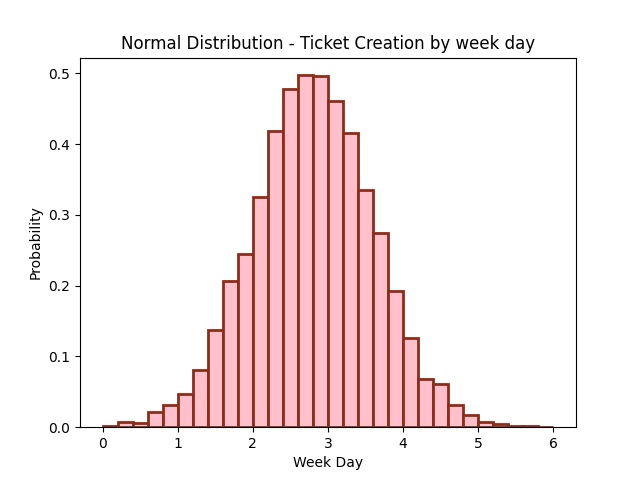
\includegraphics[width=.45\textwidth]{myplot_normal.jpg}
    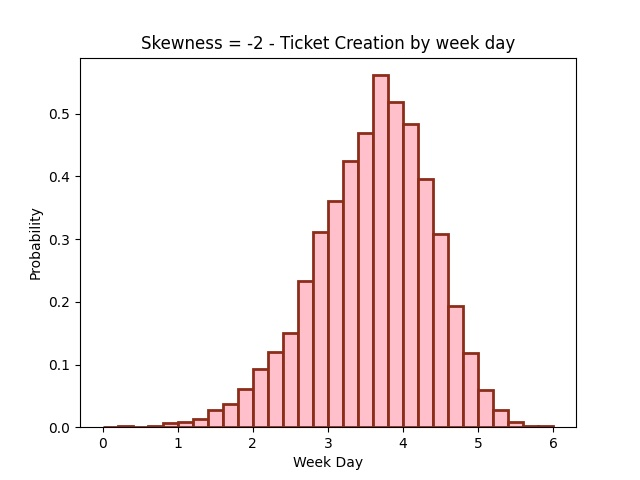
\includegraphics[width=.45\textwidth]{myplot_sk-2.jpg}
    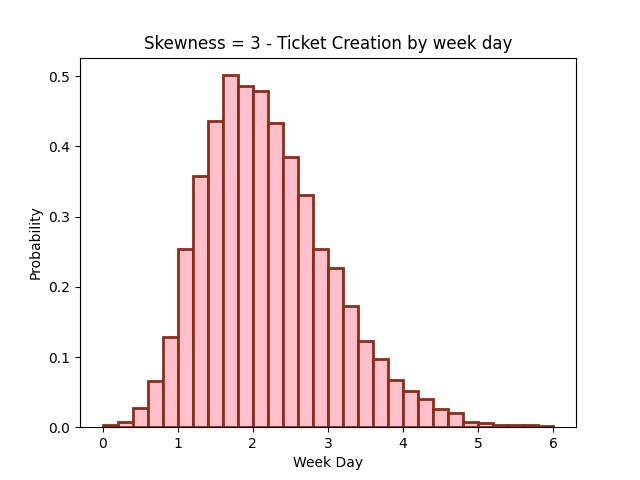
\includegraphics[width=.45\textwidth]{myplot_sk3.jpg}
    \caption{Skewness integration}
    \label{fig:skew-int}
\end{figure}

We could then move on to experimentation. Using a normal distribution, we studied the distribution of 10000 tickets generated by day of the week (0 being Sunday and 6 Saturday). We tried to influence the distribution probability by inputting a skewness value.

The results of this testing can be seen in Figure \ref{fig:skew-int}. We started by creating a normal distribution that had a skewness of 0. We changed that value to -2 and 3 and exported the end results in graphical form.

Having these outcomes, we can conclude that we can indeed generate a synthetic dataset with a chosen value of kurtosis by influencing the probability distribution of values in the generator.





%To generate skewness to either side, we just need to ensure that the mean value stays the same as it would on standard generation while shifting the mode and median to the other side. This is done by generating an extensive but focused amount of values on the opposite side of the skew while creating a spread-out number of entries on the side of the skew, generating a skewness tail on the desired side of the aisle.
\subsection{Kurtosis}

Kurtosis is a "measure of the "tailedness" of the probability distribution of a real-valued random variable" (adapted from \cite{ramya2017breast}). Like skewness, kurtosis describes the shape of a probability distribution. There are different ways of quantifying it for a theoretical distribution and corresponding ways of estimating it from a sample from a population. Other measures of kurtosis may have varied interpretations. As \cite{doi:10.1080/00031305.1988.10475539} said, and I quote: "It is best to define kurtosis vaguely as the location- and scale-free movement of probability mass from the shoulders of a distribution into its center and tails and to recognize that it can be formalized in many ways."

Kurtosis is sometimes confused with a measure of the peakedness of a distribution \citep{doi:10.1080/00031305.1970.10478885}. However, kurtosis is a measure that describes the shape of a distribution's tails concerning its overall format. All kurtosis measures are analogized against a typical normal distribution or bell curve.

\begin{figure}[!ht]
  \begin{center}
    \leavevmode
    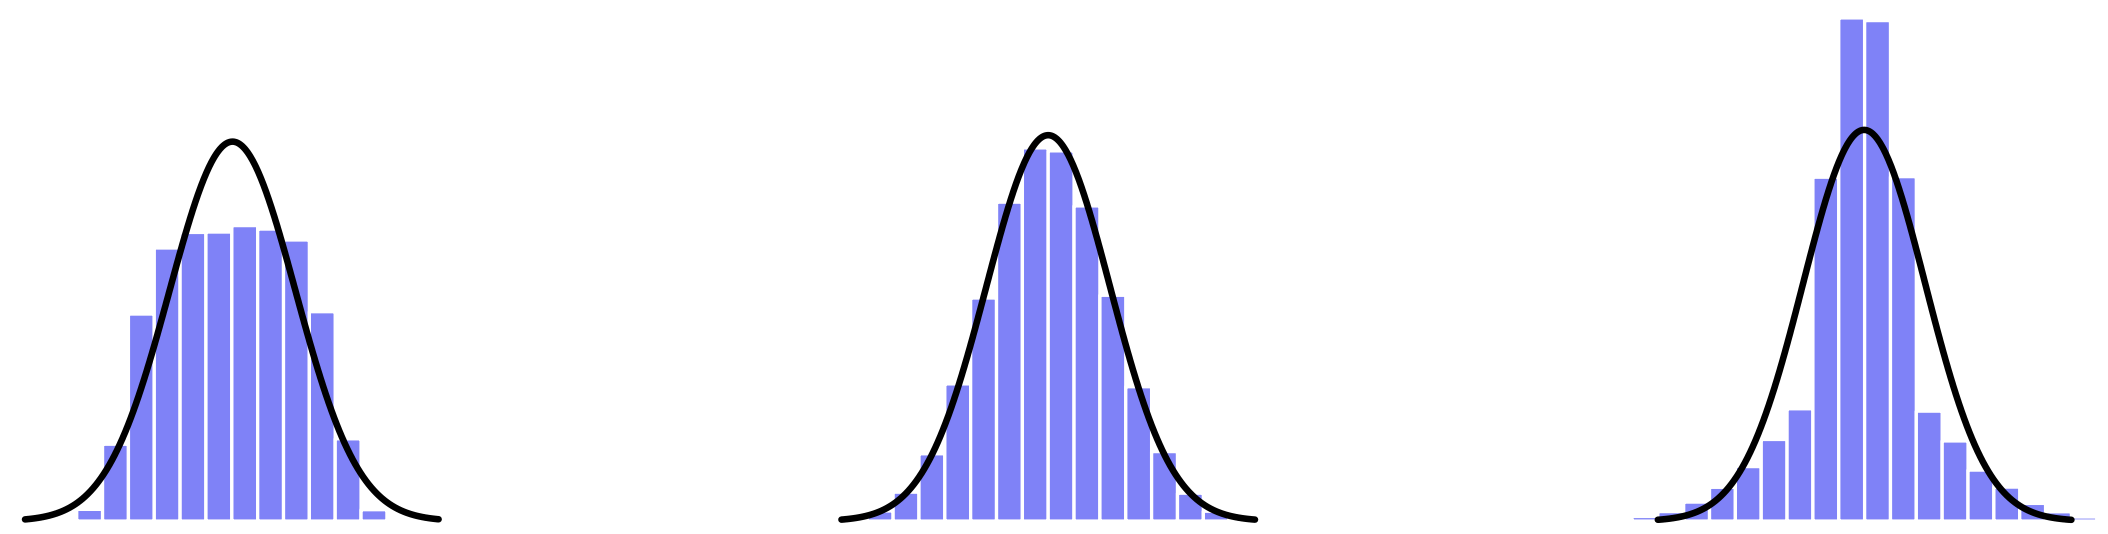
\includegraphics[width=1\textwidth]{kurtosis_histogram.png}
    \caption[Visual representation of kurtosis in histogram form]{Visual representation of kurtosis in histogram form. Removed from \cite{navarro2019learning}}
    \label{fig:kurtosis}
  \end{center}
\end{figure}

As depicted in Fig. \ref{fig:kurtosis} kurtosis can be represented in 3 types. The left graph is called a platykurtic distribution. These distributions have short tails with flattened curves. The middle graph represents a mesokurtic kurtosis distribution where kurtosis is almost exactly 0. Finally, on the right, we have a leptokurtic kurtosis, where the values of the normal distribution peak. The modal curve represented by a black curve in the figure has a kurtosis value equal to 0.

Kurtosis can be calculated using the formula \ref{eq:kurt}.
\begin{equation}
  \label{eq:kurt}
  kurt_x=\frac{m_4}{sd_x^4}-3
\end{equation}

Where $m_4$ is calculated using the formula presented in Equation \ref{eq:mj}

As with Skewness integration, adding desired kurtosis values could be done by changing the parameters of the output entries. However, influencing this value is not as easy as initially thought. Using a simple value of Kurtosis was not possible. However, we could try using different distributions and see how their Kurtosis values would influence the shape of the output dataset.
%For negative skewness, we need to reduce the number of entries closer to the mean of the distribution while assuring that output continues to be a normal distribution (only flattened in comparison to the original). Positive skewness would do the inverse, increasing the production of entries closer to the mean, creating a peak of values.

\begin{figure}[!ht]
    \centering
    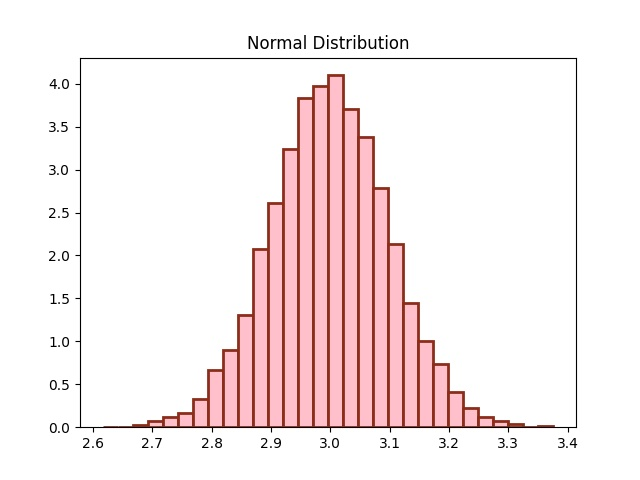
\includegraphics[width=.45\textwidth]{normal.jpg}
    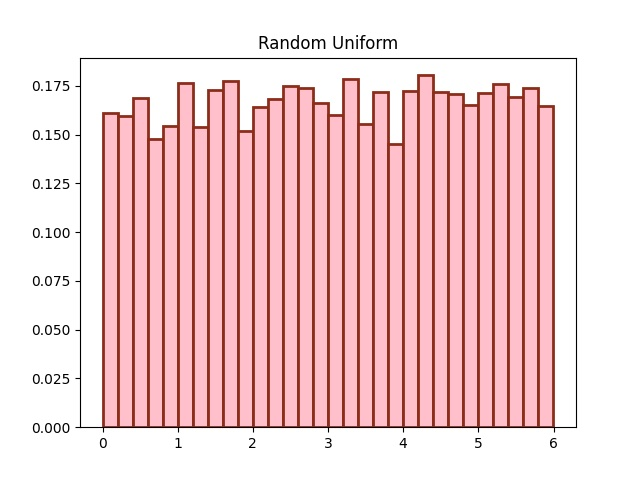
\includegraphics[width=.45\textwidth]{uniform.jpg}
    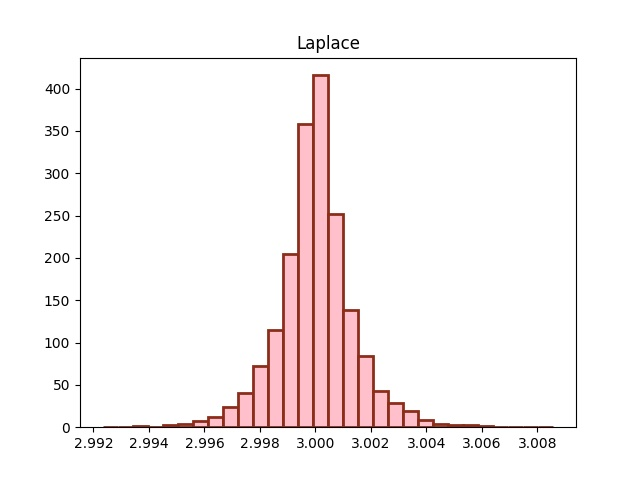
\includegraphics[width=.45\textwidth]{laplace.jpg}
    \caption{Normal, Random Uniform and Laplace distributions}
    \label{fig:kurt-int}
\end{figure}

\pagebreak
Results of this testing can be seen in Figure \ref{fig:kurt-int}. We used different distributions to generate data with distinguishable characteristics. We then calculated kurtosis on these distributions and see if its values changed according to the distribution. The uniform distribution had a kurtosis value of 1.8, Normal distribution had a value of 3. Finally, with Laplace, we arrived at a kurtosis value of 6.59.

While we found that it is possible to influence the value of kurtosis we found to way of correctly influencing that same value with a simple user input.
\section{Information-theoretic}
Information-theoretic meta features are based on entropy, capturing the data's amount of information and complexity. 
The entropy ($H_{x}$) can be given by the formula \ref{eq:if}.
\begin{equation}
  \label{eq:if}
  H_{x}=-\sum_{x=1}^{N}P_{x}log_{2}(P_{x})
\end{equation}
Where $P_{x}$ represents the probability of a category (x) to occur.

We can use this formula to calculate certain meta features in this family, such is the case of the classEnt meta feature.

Solving this problem to force a specific entropy value is a mathematical one that exceeds our capabilities. Nevertheless, from an engineering standpoint, we propose the analysis of entropy at set intervals during the generation process. For each gap, we would freeze the generation, calculate entropy and see how far we are from our target. In cases where values are superior to the desired ones, we should try to generate more noise, reducing the more significant percentages and lowering the entropy. In cases where we were already lower, we should focus the generation on existing, more probable values. This would increase their final probability and levelling our entropy values. 

Would setting a particular value of entropy be helpful to the final dataset? In a simple answer, yes. Entropy measures disorder or impurities in the information processed in machine learning. The ability to choose that purity level has obvious benefits from an ML study standpoint.

\section{Landmarking}
We arrived at strange conclusions regarding landmarking meta features when analysing possible meta features to validate their inclusion in synthetic dataset generation processes. These meta features use algorithms to characterise datasets. To include specific values of these meta features, we would need to create entries while also knowing how well the entire dataset would behave when fronting said algorithm.

A funny analogy to this problem would be to drive a train while building the train tracks, taking into account the performance of every vehicle on the railroad system. The complexity of this problem vastly overshadows the scope of this study.

Landmarking inclusion would be rather valuable, especially in machine learning cases. Users could generate datasets with good and bad results, teaching the MLM to follow datasets with good results. However, their inclusion could prove troublesome as data could serve the dataset too perfectly. 

Generating datasets with set algorithmic results would lead to synthetic datasets riddled with overfitting problems.

\section{Dataset Morphing}
One option we came across to use to create datasets with specific values of meta features was dataset morphing. With dataset morphing, we could change it after having a complete dataset and altering its values to achieve the desired meta feature value results.

This, however, comes with a set of problems. Let's use the same case we already used with kurtosis and skewness. So we want to alter the ticket generation time by day of the week. To do this, we need to finish the generation process and then change the data on columns related to that information. This change also needs to impact the rest of the dataset, not just that one column. The generation process would need to be halted in columns whose data depends on the morphed columns. Only after the data connected to the morphing finishes being generated and is morphed can the generation process continue.

This process is more time and resource expensive than normal run-time generation.
\section{Conclusion}
In this chapter, we looked at the original approach taken to test some of the methodologies later described in the chapter. 

We then analysed some possible meta feature inclusions to the generation process. We explored the possibility of including general, statistical, information-theoretic and landmarking meta features. We also looked at the validity of incorporating these meta features in each analysis.

We also looked at the possibility of dataset morphing to insert meta feature values into a synthetic dataset.

While we found it possible to insert meta features, we did it in a singular factor. By inserting a meta feature, we cannot guarantee that the values of other meta features in the dataset will be maintained.

Datasets generated with dataset integration, be it by runtime integration or morphing should them be analysed to see if they continue to be valid and realistic. A debugging analysis should be made, in order to guarantee the stability of buisiness rules inside the dataset to guarantee the validity of the data. Some of the data evaluation methods described in Chapter \ref{chap:generation} should also be used to check the validity of the final output.

When looking at what was achieved in this part of the study and what was initially idealised, it is impossible not to feel underwhelmed. We analysed ways to force certain meta features into the generation process. We proved that this implementation can be done on simple and statistical meta features. We conclude that a complete study on the subject should be made to get to any plausible conclusion on including meta features with more complicated calculations.
\chapter{Conclusion}
\label{chap:Conclusion}

During the development of this study, we tried to tackle the theme of 'Meta Feature classification and insertion on a Synthetic dataset generation process.' With SNOOKER as the original basis, we analyzed the concept of meta features, exploring the subject and presenting the most commonly known family of meta features. While groups of meta features are not uniformly described, the list presentive is extensive and varied enough to characterize a dataset correctly.

The study advanced to dataset generation methodologies. While explored, this subject was not developed further during the development phase.

The Classification feature was appended to SNOOKER. We used the pyfme library to help us extract as many meta features from generated datasets as possible, allowing for vast classification options.

We also explored ways to force specific meta feature results on synthetic datasets. Due to a lack of practical results, our observations were purely theoretical, having no sound proof to correctly evaluate our hypotheses. While we believed that inserting meta features into synthetic datasets is a possible and (in some cases) beneficial endeavour, no testing was finalized.

The development of this study went through more problems than expected. The meta-extraction tool ended up occupying most of the time available for development. There is also an evident lack of knowledge and know-how regarding dataset analysis and generation processes that hindered the development and limited the scope of the study. 

\section{Future Works}
As said before, the study of meta feature inclusion on generation could benefit from further research, being a possible project to be.

We can now classificate datasets using the meta feature classification tool. We could test performance on machine learning models trained using similar datasets with different meta feature values. This is also an interesting topic that requires further research.

Lastly, we present possible advances to SNOOKER as a product. After exploring SNOOKER, it is easy to see that computing power and runtime are essential factors needed when dealing with the generator. We conclude that SNOOKER would profit from a significant overhaul, becoming decentralized. Having all the necessary calculations done remotely on a server. As meta-analysis of some families could take a long time, making them run in a server would prevent users from needing to keep processes running for long times. The results could be sent to the user at a later date. We conclude that SNOOKER would benefit from evolving into a web service.


%%----------------------------------------
%% Final materials
%%----------------------------------------

%% Bibliography
%% Comment the next command if BibTeX file not used
%% bibliography is in ``myrefs.bib''
\PrintBib{myrefs}

%% 2021-07-20: change
%% comment next 2 commands if numbered appendices are not used
\appendix
\chapter{SNOOKER Synthetic Dataset} \label{ap3:snooker}
In this appendix, we will look at the final output from SNOOKER’s generation process, explaining the information in each dataset column. Columns can be classified as primary and secondary. While primary columns display information essential for the dataset, secondary columns facilitate debugging actions. Other columns exist when generating datasets for different ends. Still, the study and analysed are based only on the helpdesk dataset type output. When looking at the 1st line of the CSV file (the header), we can extract all the columns that will be analysed:

\begin{lstlisting}[breaklines=true]
  ID; Location; Raised (UTC); Allocated; Stages; Fixed; Client; Family; Family Action; Subfamily; Subfamily Action; Subfamily Action Duration; Team; Users in the Shift; Users Next Shift; Users Competent; User actions; User Chosen; Action Chosen; Action Chosen Status; Action Chosen Duration; Action Chosen (With Outlier); Ticket Duration; Escalate; Status; Outlier

\end{lstlisting}

The first column displays the ticket's ID, a unique numerical identifier; in this case, the ID is also the ticket's number. The second column contains the location of the ticket (its country of origin). Raised (UTC) displays the DateTime the ticket was submitted in UTC format. At the same time, the next column (Allocated) does the same for the time the ticket was allocated to a helpdesk team member. 

Stages register many timestamps concerning the ticket treatment. Fixed, like Allocated did before, keeps the DateTime tickets solved. The next metric is simple: the Client column gives information regarding the client the ticket belongs to.

Family, Family Action, Subfamily and Subfamily Action characteristics keep information regarding the nature of the incident that caused that ticket. The Actions metrics save the techniques usually used to solve those problems. Lastly, the Subfamily Action Duration illustrates the time needed to perform the actions presented in the Subfamily Action column.

Team, Users in the Shift and Users Next Shift give information regarding the team management, the current team, its active members and the members that will become available during the next shift, respectively. Users competent present a list of the most suitable member to perform the task. The User actions column contains data regarding the action that each available user would perform. User Chosen presents us with the team member that will take care of the ticket. Action Chosen reflects the action chosen to fix the incident, followed by the Action Chosen Status that represents the status of the action chosen. Action Chosen Duration and Action Chosen Duration (With Outlier) display the action's duration and duration if an outlier exists.

The final four columns are Ticket Duration, Escalate, Status and Outlier. The first one depicts the time the ticket has endured without being solved, followed by Escalate, responsible for informing the user that the ticket should be passed to the next team. The Status column provides the ticket status (Closed or Transferred). Finally, the Outlier notifies us if the ticket should be considered an outlier.
\chapter{Pymfe Meta feature tables} \label{ap1:pymfe_mf}

\begin{table}[h!]
  \centering
  \caption{Pymfe general meta features}
  \setlength{\tabcolsep}{8pt}
  \renewcommand{\arraystretch}{1.2}
  \begin{tabular}{lll}
    \hline
    Family & Meta Feature & Description \\ \hline
  general & attr\_to\_inst & Compute the ratio between the number of attributes.\\
  general & cat\_to\_num & Compute the ratio between the number of \\ & & categoric and numeric features.\\
  general & freq\_class & Compute the relative frequency of each distinct class.\\
  general & inst\_to\_attr & Compute the ratio between the number of instances\\ & & and attributes.\\
  general & nr\_attr & Compute the total number of attributes.\\
  general & nr\_bin & Compute the number of binary attributes.\\
  general & nr\_cat & Compute the number of categorical attributes.\\
  general & nr\_class & Compute the number of distinct classes.\\
  general & nr\_inst & Compute the number of instances (rows) in the dataset.\\
  general & nr\_num & Compute the number of numeric features.\\
  general & num\_to\_cat & Compute the number of numerical and categorical features. \\ \hline
  \end{tabular}
  \label{tab:pymfe-general-mf}
\end{table}

\begin{table}[h!]
  \centering
  \caption{Pymfe statistical meta features}
  \setlength{\tabcolsep}{8pt}
  \renewcommand{\arraystretch}{1.2}
  \begin{tabular}{lll}
    \hline
    Family & Meta Feature & Description \\ \hline
    statistical & can\_cor & Compute canonical correlations of data.\\
    statistical & cor & Compute the absolute value of the correlation of distinct dataset\\ & & column pairs.\\
    statistical & cov & Compute the absolute value of the covariance of distinct dataset\\ & & attribute pairs.\\
    statistical & eigenvalues & Compute the eigenvalues of covariance matrix from dataset.\\
    statistical & g\_mean & Compute the geometric mean of each attribute.\\
    statistical & gravity & Compute the distance between minority and majority classes\\ & & center of mass.\\
    statistical & h\_mean & Compute the harmonic mean of each attribute.\\
    statistical & iq\_range & Compute the interquartile range (IQR) of each attribute.\\
    statistical & kurtosis & Compute the kurtosis of each attribute.\\
    statistical & lh\_trace & Compute the Lawley-Hotelling trace.\\
    statistical & mad & Compute the Median Absolute Deviation (MAD) adjusted by a\\ & & factor.\\
    statistical & max & Compute the maximum value from each attribute.\\
    statistical & mean & Compute the mean value of each attribute.\\
    statistical & median & Compute the median value from each attribute.\\
    statistical & min & Compute the minimum value from each attribute.\\
    statistical & nr\_cor\_attr & Compute the number of distinct highly correlated pair\\ & & of attributes.\\
    statistical & nr\_disc & Compute the number of canonical correlation between each\\ & & attribute and class.\\
    statistical & nr\_norm & Compute the number of attributes normally distributed based\\ & & in a given method.\\
    statistical & nr\_outliers & Compute the number of attributes with at least one outlier value.\\
    statistical & p\_trace & Compute the Pillai’s trace.\\
    statistical & range & Compute the range (max - min) of each attribute.\\
    statistical & roy\_root & Compute the Roy’s largest root.\\
    statistical & sd & Compute the standard deviation of each attribute.\\
    statistical & sd\_ratio & Compute a statistical test for homogeneity of covariances.\\
    statistical & skewness & Compute the skewness for each attribute.\\
    statistical & sparsity & Compute (possibly normalized) sparsity metric for each attribute.\\
    statistical & t\_mean & Compute the trimmed mean of each attribute.\\
    statistical & var & Compute the variance of each attribute.\\
    statistical & w\_lambda & Compute the Wilks’ Lambda value.\\\hline
  \end{tabular}
  \label{tab:pymfe-statistical-mf}
\end{table}

\begin{table}[h!]
  \centering
  \caption{Pymfe Information-theoretic meta features}
  \setlength{\tabcolsep}{8pt}
    \renewcommand{\arraystretch}{1.2}
      \begin{tabular}{lll}
        \hline
      Family & Meta Feature & Description \\
      \hline
      info-theory & attr\_conc & Compute concentration coef. of each pair of distinct attributes.\\
      info-theory & attr\_ent & Compute Shannon’s entropy for each predictive attribute.\\
      info-theory & class\_conc & Compute concentration coefficient between each attribute\\ & & and class.\\
      info-theory & class\_ent & Compute target attribute Shannon’s entropy.\\
      info-theory & eq\_num\_attr & Compute the number of attributes equivalent for a predictive\\ & & task.\\
      info-theory & joint\_ent & Compute the joint entropy between each attribute and class.\\
      info-theory & mut\_inf & Compute the mutual information between each attribute and\\ & & target.\\
      info-theory & ns\_ratio & Compute the noisiness of attributes.\\\hline
  \end{tabular}
  \label{tab:pymfe-it-mf}
\end{table}

\begin{table}[h!]
  \centering
  \caption{Pymfe Model-based meta features}
  \setlength{\tabcolsep}{8pt}
    \renewcommand{\arraystretch}{1.2}
      \begin{tabular}{lll}
        \hline
      Family & Meta Feature & Description \\
      \hline
      model-based & leaves & Compute the number of leaf nodes in the DT model.\\
      model-based & leaves\_branch & Compute the size of branches in the DT model.\\
      model-based & leaves\_corrob & Compute the leaves corroboration of the DT model.\\
      model-based & leaves\_homo & Compute the DT model Homogeneity for every leaf node.\\
      model-based & leaves\_per\_class & Compute the proportion of leaves per class in DT model.\\
      model-based & nodes & Compute the number of non-leaf nodes in DT model.\\
      model-based & nodes\_per\_attr & Compute the ratio of nodes per number of attributes in\\ & & DT model.\\
      model-based & nodes\_per\_inst & Compute the ratio of non-leaf nodes per number of \\ & & instances in DT model.\\
      model-based & nodes\_per\_level & Compute the ratio of number of nodes per tree level in\\ & & DT model.\\
      model-based & nodes\_repeated & Compute the number of repeated nodes in DT model.\\
      model-based & tree\_depth & Compute the depth of every node in the DT model.\\
      model-based & tree\_imbalance & Compute the tree imbalance for each leaf node.\\
      model-based & tree\_shape & Compute the tree shape for every leaf node.\\
      model-based & var\_importance & Compute the features importance of the DT model for\\ & & each attribute.\\\hline
  \end{tabular}
  \label{tab:pymfe-mb-mf}
\end{table}

\begin{table}[h!]
  \centering
  \caption{Pymfe Landmarking meta features}
  \setlength{\tabcolsep}{8pt}
    \renewcommand{\arraystretch}{1.2}
      \begin{tabular}{lll}
        \hline
      Family & Meta Feature & Description \\
      \hline
      landmarking & best\_node & Performance of a the best single decision tree node.\\
      landmarking & elite\_nn & Performance of Elite Nearest Neighbor.\\
      landmarking & linear\_discr & Performance of the Linear Discriminant classifier.\\
      landmarking & naive\_bayes & Performance of the Naive Bayes classifier.\\
      landmarking & one\_nn & Performance of the 1-Nearest Neighbor classifier.\\
      landmarking & random\_node & Performance of the single decision tree node\\ & & model induced by a random attribute.\\
      landmarking & worst\_node & Performance of the single decision tree node\\ & & model induced by the worst informative attribute.\\\hline
  \end{tabular}
  \label{tab:pymfe-landmarking-mf}
\end{table}

\begin{table}[h!]
  \centering
  \caption{Pymfe Clustering meta features}
  \setlength{\tabcolsep}{8pt}
    \renewcommand{\arraystretch}{1.2}
      \begin{tabular}{lll}
      \hline
      Family & Meta Feature & Description \\ \hline
      clustering & ch & Compute the Calinski and Harabasz index. \\
      clustering & int & Compute the INT index.\\
      clustering & nre & Compute the normalized relative entropy.\\
      clustering & pb & Compute the pearson correlation between \\
      & & class matching and instance distances.\\
      clustering & sc & Compute the number of clusters with\\ & & size smaller than a given size.\\
      clustering & sil & Compute the mean silhouette value.\\
      clustering & vdb & Compute the Davies and Bouldin Index.\\
      clustering & vdu & Compute the Dunn Index.\\ \hline
    \end{tabular}
    \label{tab:pymfe-clustering-mf}
  \end{table}

   \begin{table}[h!]
    \centering
    \caption{Pymfe concept meta features}
    \setlength{\tabcolsep}{8pt}
      \renewcommand{\arraystretch}{1.2}
        \begin{tabular}{lll}
          \hline
          Family & Meta Feature & Description \\ \hline
        concept & cohesiveness & Compute the improved version of the weighted distance,\\ & & that captures how dense or sparse is the example distribution.\\
        concept & conceptvar & Compute the concept variation that estimates the variability\\ & & of class labels among examples.\\
        concept & impconceptvar & Compute the improved concept variation that estimates the\\ & & variability of class labels among examples.\\
        concept & wg\_dist & Compute the weighted distance, that captures how dense or\\ & & sparse is the example distribution.\\\hline
    \end{tabular}
    \label{tab:pymfe-concept-mf}
  \end{table}

  \begin{table}[h!]
    \centering
    \caption{Pymfe itemset meta features}
    \setlength{\tabcolsep}{8pt}
      \renewcommand{\arraystretch}{1.2}
        \begin{tabular}{lll}
          \hline
          Family & Meta Feature & Description \\ \hline
          itemset & one\_itemset & Compute the one itemset meta feature.\\          
          itemset & two\_itemset & Compute the two itemset meta feature.\\\hline

    \end{tabular}
    \label{tab:pymfe-itemset-mf}
  \end{table}

  \begin{table}[h!]
    \centering
    \caption{Pymfe complexity meta features}
    \setlength{\tabcolsep}{8pt}
      \renewcommand{\arraystretch}{1.2}
        \begin{tabular}{lll}
        \hline
        Family & Meta Feature & Description \\ \hline
      complexity & c & Compute the entropy of class proportions.\\
      complexity & c2 & Compute the imbalance ratio.\\
      complexity & cls\_coef & Clustering coefficient.\\
      complexity & density & Average density of the network.\\
      complexity & f1 & Maximum Fisher's discriminant ratio.\\
      complexity & f1v & Directional-vector maximum Fisher's \\ & & discriminant ratio.\\
      complexity & f2 & Volume of the overlapping region.\\
      complexity & f3 & Compute feature maximum individual \\ & & efficiency.\\
      complexity & f4 & Compute the collective feature efficiency.\\
      complexity & hubs & Hub score.\\
      complexity & l1 & Sum of error distance by linear programming.\\
      complexity & l2 & Compute the OVO subsets error rate of\\ & & linear classifier.\\
      complexity & l3 & Non-Linearity of a linear classifier.\\
      complexity & lsc & Local set average cardinality.\\
      complexity & n1 & Compute the fraction of borderline \\ & &points.\\
      complexity & n2 & Ratio of intra and extra class nearest\\ & & neighbor distance.\\
      complexity & n3 & Error rate of the nearest neighbor classifier.\\
      complexity & n4 & Compute the non-linearity of the k-NN Classifier.\\
      complexity & t1 & Fraction of hyperspheres covering data.\\
      complexity & t2 & Compute the average number of features \\ & &per dimension.\\
      complexity & t3 & Compute the average number of PCA \\ & &dimensions per points.\\
      complexity & t4 & Compute the ratio of the PCA dimension \\ & & to the original dimension.\\\hline
    \end{tabular}
    \label{tab:pymfe-complexity-mf}
  \end{table}
\chapter{Meta Analysis Output} \label{ap2:meta_files}

Statistical meta feature analysis output file:
\begin{lstlisting}[breaklines=true, basicstyle=\footnotesize, tabsize=1]
  Statistical Meta Feature Analysis of file in /Users/joaolemos/DatasetGen/Output/Generation/test.csv at 2022-06-02 00:15:09.428844.
  can_cor.mean                    1.0
  can_cor.sd                      2.863353569008059e-16
  cor.mean                        0.0031818656040018055
  cor.sd                          0.029273671606693415
  cov.mean                        0.00018169921467679913
  cov.sd                          0.06544132326412351
  eigenvalues.mean                8.517833528021107
  eigenvalues.sd                  584.2881540682121
  g_mean.mean                     0.02200758566217588
  g_mean.sd                       0.8030517936688358
  gravity                         14.491376746189438
  h_mean.mean                     0.017814411761191074
  h_mean.sd                       0.6219661342834908
  iq_range.mean                   0.018441748588161472
  iq_range.sd                     0.6913274616349807
  kurtosis.mean                   878.1186853398123
  kurtosis.sd                     283.23712818907694
  lh_trace                        inf
  mad.mean                        0.009141821376281114
  mad.sd                          0.35732979367673556
  max.mean                        1.3132189918427106
  max.sd                          19.345451307983584
  mean.mean                       0.0399734463403152
  mean.sd                         1.6495148276889133
  median.mean                     0.01930767621836436
  median.sd                       0.6700330673798763
  min.mean                        0.006065676636686885
  min.sd                          0.21001299789299555
  nr_cor_attr                     0.0007765221295242062
  nr_disc                         1000
  nr_norm                         0.0
  nr_outliers                     4774
  p_trace                         999.9999999999998
  range.mean                      1.3071533152060237
  range.sd                        19.23267679677396
  roy_root                        inf
  sd.mean                         0.08891679211579023
  sd.sd                           2.9174831022006753
  sd_ratio                        nan
  skewness.mean                   28.866039090472135
  skewness.sd                     6.782417085249947
  sparsity.mean                   0.13476022492442502
  sparsity.sd                     0.19501828184302594
  t_mean.mean                     0.02068489003024659
  t_mean.sd                       0.7202330927954221
  var.mean                        8.517833528021098
  var.sd                          584.2706323926961
  w_lambda                        0.0
  
  Analysis took 0:28:16.250728.
  
\end{lstlisting}
\chapter{Statistical Analysis Output} \label{appendix:statistical}

\begin{lstlisting}[breaklines=true, basicstyle=\footnotesize, tabsize=1]
Analysis of file ../../Output/generatedDatasets/SD1.csv.
can_cor.mean                  1.0
can_cor.sd                    2.863353569008059e-16
Analysis took 0:26:32.801149.
cor.mean                      0.0031818656040018055
cor.sd                        0.029273671606693415
Analysis took 0:27:16.633176.
cov.mean                      0.00018169921467679913
cov.sd                        0.06544132326412351
Analysis took 0:25:29.343186.
eigenvalues.mean              8.517833528021107
eigenvalues.sd                584.2881540682121
Analysis took 0:31:03.024574.
g_mean.mean                   0.02200758566217588
g_mean.sd                     0.8030517936688358
Analysis took 0:25:42.758934.
gravity                       14.491376746189438
Analysis took 0:26:54.196286.
h_mean.mean                   0.017814411761191074
h_mean.sd                     0.6219661342834908
Analysis took 0:25:32.138877.
iq_range.mean                 0.018441748588161472
iq_range.sd                   0.6913274616349807
Analysis took 0:27:45.718662.
kurtosis.mean                 878.1186853398123
kurtosis.sd                   283.23712818907694
Analysis took 0:26:54.988853.
lh_trace                      inf
Analysis took 0:26:04.834030.
mad.mean                      0.009141821376281114
mad.sd                        0.35732979367673556
Analysis took 0:28:52.903699.
max.mean                      1.3132189918427106
max.sd                        19.345451307983584
Analysis took 0:26:29.736283.
mean.mean                     0.0399734463403152
mean.sd                       1.6495148276889133
Analysis took 0:26:56.504050.
median.mean                   0.01930767621836436
median.sd                     0.6700330673798763
Analysis took 0:27:36.376224.
min.mean                      0.006065676636686885
min.sd                        0.21001299789299555
Analysis took 0:26:31.345163.
nr_cor_attr                   0.0007765221295242062
Analysis took 0:47:58.595005.
nr_disc                       1000
Analysis took 0:27:54.741807.
nr_norm                       0.0
Analysis took 0:27:40.943515.
nr_outliers                   4774
Analysis took 0:24:35.350784.
p_trace                       999.9999999999998
Analysis took 0:24:35.025303.
range.mean                    1.3071533152060237
range.sd                      19.23267679677396
Analysis took 0:35:49.239344.
roy_root                      inf
Analysis took 0:26:51.358588.
sd.mean                       0.08891679211579023
sd.sd                         2.9174831022006753
Analysis took 0:26:14.329449.
sd_ratio                      nan
Analysis took 0:27:26.405710.
skewness.mean                 28.866039090472135
skewness.sd                   6.782417085249947
Analysis took 0:24:42.426164.
sparsity.mean                 0.13476022492442502
sparsity.sd                   0.19501828184302594
Analysis took 0:27:49.408391.
var.mean                      8.517833528021098
var.sd                        584.2706323926961
Analysis took 0:24:23.294747.
w_lambda                      0.0
Analysis took 0:23:56.400821.
\end{lstlisting}

%% Index
%% Uncomment next command if index is required
%% don't forget to run ``makeindex thesis'' command
%\PrintIndex

\end{document}
